

% \begin{figure*}[b]
%     %\centering
%     \begin{subfigure}{0.48\textwidth}
%         \centering
%          \resizebox{\textwidth}{!}{%% Creator: Matplotlib, PGF backend
%%
%% To include the figure in your LaTeX document, write
%%   \input{<filename>.pgf}
%%
%% Make sure the required packages are loaded in your preamble
%%   \usepackage{pgf}
%%
%% Also ensure that all the required font packages are loaded; for instance,
%% the lmodern package is sometimes necessary when using math font.
%%   \usepackage{lmodern}
%%
%% Figures using additional raster images can only be included by \input if
%% they are in the same directory as the main LaTeX file. For loading figures
%% from other directories you can use the `import` package
%%   \usepackage{import}
%%
%% and then include the figures with
%%   \import{<path to file>}{<filename>.pgf}
%%
%% Matplotlib used the following preamble
%%   \def\mathdefault#1{#1}
%%   \everymath=\expandafter{\the\everymath\displaystyle}
%%   
%%   \makeatletter\@ifpackageloaded{underscore}{}{\usepackage[strings]{underscore}}\makeatother
%%
\begingroup%
\makeatletter%
\begin{pgfpicture}%
\pgfpathrectangle{\pgfpointorigin}{\pgfqpoint{6.474692in}{4.420679in}}%
\pgfusepath{use as bounding box, clip}%
\begin{pgfscope}%
\pgfsetbuttcap%
\pgfsetmiterjoin%
\definecolor{currentfill}{rgb}{1.000000,1.000000,1.000000}%
\pgfsetfillcolor{currentfill}%
\pgfsetlinewidth{0.000000pt}%
\definecolor{currentstroke}{rgb}{1.000000,1.000000,1.000000}%
\pgfsetstrokecolor{currentstroke}%
\pgfsetdash{}{0pt}%
\pgfpathmoveto{\pgfqpoint{0.000000in}{0.000000in}}%
\pgfpathlineto{\pgfqpoint{6.474692in}{0.000000in}}%
\pgfpathlineto{\pgfqpoint{6.474692in}{4.420679in}}%
\pgfpathlineto{\pgfqpoint{0.000000in}{4.420679in}}%
\pgfpathlineto{\pgfqpoint{0.000000in}{0.000000in}}%
\pgfpathclose%
\pgfusepath{fill}%
\end{pgfscope}%
\begin{pgfscope}%
\pgfsetbuttcap%
\pgfsetmiterjoin%
\definecolor{currentfill}{rgb}{1.000000,1.000000,1.000000}%
\pgfsetfillcolor{currentfill}%
\pgfsetlinewidth{0.000000pt}%
\definecolor{currentstroke}{rgb}{0.000000,0.000000,0.000000}%
\pgfsetstrokecolor{currentstroke}%
\pgfsetstrokeopacity{0.000000}%
\pgfsetdash{}{0pt}%
\pgfpathmoveto{\pgfqpoint{0.374692in}{0.320679in}}%
\pgfpathlineto{\pgfqpoint{6.374692in}{0.320679in}}%
\pgfpathlineto{\pgfqpoint{6.374692in}{4.320679in}}%
\pgfpathlineto{\pgfqpoint{0.374692in}{4.320679in}}%
\pgfpathlineto{\pgfqpoint{0.374692in}{0.320679in}}%
\pgfpathclose%
\pgfusepath{fill}%
\end{pgfscope}%
\begin{pgfscope}%
\pgfpathrectangle{\pgfqpoint{0.374692in}{0.320679in}}{\pgfqpoint{6.000000in}{4.000000in}}%
\pgfusepath{clip}%
\pgfsetbuttcap%
\pgfsetroundjoin%
\definecolor{currentfill}{rgb}{0.121569,0.466667,0.705882}%
\pgfsetfillcolor{currentfill}%
\pgfsetlinewidth{1.003750pt}%
\definecolor{currentstroke}{rgb}{0.121569,0.466667,0.705882}%
\pgfsetstrokecolor{currentstroke}%
\pgfsetdash{}{0pt}%
\pgfsys@defobject{currentmarker}{\pgfqpoint{-0.012028in}{-0.012028in}}{\pgfqpoint{0.012028in}{0.012028in}}{%
\pgfpathmoveto{\pgfqpoint{0.000000in}{-0.012028in}}%
\pgfpathcurveto{\pgfqpoint{0.003190in}{-0.012028in}}{\pgfqpoint{0.006250in}{-0.010761in}}{\pgfqpoint{0.008505in}{-0.008505in}}%
\pgfpathcurveto{\pgfqpoint{0.010761in}{-0.006250in}}{\pgfqpoint{0.012028in}{-0.003190in}}{\pgfqpoint{0.012028in}{0.000000in}}%
\pgfpathcurveto{\pgfqpoint{0.012028in}{0.003190in}}{\pgfqpoint{0.010761in}{0.006250in}}{\pgfqpoint{0.008505in}{0.008505in}}%
\pgfpathcurveto{\pgfqpoint{0.006250in}{0.010761in}}{\pgfqpoint{0.003190in}{0.012028in}}{\pgfqpoint{0.000000in}{0.012028in}}%
\pgfpathcurveto{\pgfqpoint{-0.003190in}{0.012028in}}{\pgfqpoint{-0.006250in}{0.010761in}}{\pgfqpoint{-0.008505in}{0.008505in}}%
\pgfpathcurveto{\pgfqpoint{-0.010761in}{0.006250in}}{\pgfqpoint{-0.012028in}{0.003190in}}{\pgfqpoint{-0.012028in}{0.000000in}}%
\pgfpathcurveto{\pgfqpoint{-0.012028in}{-0.003190in}}{\pgfqpoint{-0.010761in}{-0.006250in}}{\pgfqpoint{-0.008505in}{-0.008505in}}%
\pgfpathcurveto{\pgfqpoint{-0.006250in}{-0.010761in}}{\pgfqpoint{-0.003190in}{-0.012028in}}{\pgfqpoint{0.000000in}{-0.012028in}}%
\pgfpathlineto{\pgfqpoint{0.000000in}{-0.012028in}}%
\pgfpathclose%
\pgfusepath{stroke,fill}%
}%
\begin{pgfscope}%
\pgfsys@transformshift{0.647419in}{4.138861in}%
\pgfsys@useobject{currentmarker}{}%
\end{pgfscope}%
\begin{pgfscope}%
\pgfsys@transformshift{0.672789in}{4.138861in}%
\pgfsys@useobject{currentmarker}{}%
\end{pgfscope}%
\begin{pgfscope}%
\pgfsys@transformshift{0.698159in}{4.138861in}%
\pgfsys@useobject{currentmarker}{}%
\end{pgfscope}%
\begin{pgfscope}%
\pgfsys@transformshift{0.723529in}{4.138861in}%
\pgfsys@useobject{currentmarker}{}%
\end{pgfscope}%
\begin{pgfscope}%
\pgfsys@transformshift{0.748899in}{4.138861in}%
\pgfsys@useobject{currentmarker}{}%
\end{pgfscope}%
\begin{pgfscope}%
\pgfsys@transformshift{0.774269in}{4.138861in}%
\pgfsys@useobject{currentmarker}{}%
\end{pgfscope}%
\begin{pgfscope}%
\pgfsys@transformshift{0.799639in}{4.138861in}%
\pgfsys@useobject{currentmarker}{}%
\end{pgfscope}%
\begin{pgfscope}%
\pgfsys@transformshift{0.825009in}{4.138861in}%
\pgfsys@useobject{currentmarker}{}%
\end{pgfscope}%
\begin{pgfscope}%
\pgfsys@transformshift{0.850379in}{4.138861in}%
\pgfsys@useobject{currentmarker}{}%
\end{pgfscope}%
\begin{pgfscope}%
\pgfsys@transformshift{0.875749in}{4.138861in}%
\pgfsys@useobject{currentmarker}{}%
\end{pgfscope}%
\begin{pgfscope}%
\pgfsys@transformshift{0.901119in}{4.138861in}%
\pgfsys@useobject{currentmarker}{}%
\end{pgfscope}%
\begin{pgfscope}%
\pgfsys@transformshift{0.926489in}{4.138861in}%
\pgfsys@useobject{currentmarker}{}%
\end{pgfscope}%
\begin{pgfscope}%
\pgfsys@transformshift{0.951859in}{4.138861in}%
\pgfsys@useobject{currentmarker}{}%
\end{pgfscope}%
\begin{pgfscope}%
\pgfsys@transformshift{0.977229in}{4.138861in}%
\pgfsys@useobject{currentmarker}{}%
\end{pgfscope}%
\begin{pgfscope}%
\pgfsys@transformshift{1.002599in}{4.138861in}%
\pgfsys@useobject{currentmarker}{}%
\end{pgfscope}%
\begin{pgfscope}%
\pgfsys@transformshift{1.027969in}{4.138861in}%
\pgfsys@useobject{currentmarker}{}%
\end{pgfscope}%
\begin{pgfscope}%
\pgfsys@transformshift{1.053339in}{4.138861in}%
\pgfsys@useobject{currentmarker}{}%
\end{pgfscope}%
\begin{pgfscope}%
\pgfsys@transformshift{1.078709in}{4.138861in}%
\pgfsys@useobject{currentmarker}{}%
\end{pgfscope}%
\begin{pgfscope}%
\pgfsys@transformshift{1.104079in}{4.138861in}%
\pgfsys@useobject{currentmarker}{}%
\end{pgfscope}%
\begin{pgfscope}%
\pgfsys@transformshift{1.129449in}{4.138861in}%
\pgfsys@useobject{currentmarker}{}%
\end{pgfscope}%
\begin{pgfscope}%
\pgfsys@transformshift{1.154819in}{4.138861in}%
\pgfsys@useobject{currentmarker}{}%
\end{pgfscope}%
\begin{pgfscope}%
\pgfsys@transformshift{1.180189in}{4.138861in}%
\pgfsys@useobject{currentmarker}{}%
\end{pgfscope}%
\begin{pgfscope}%
\pgfsys@transformshift{1.205559in}{4.138861in}%
\pgfsys@useobject{currentmarker}{}%
\end{pgfscope}%
\begin{pgfscope}%
\pgfsys@transformshift{1.230929in}{4.138861in}%
\pgfsys@useobject{currentmarker}{}%
\end{pgfscope}%
\begin{pgfscope}%
\pgfsys@transformshift{1.256299in}{4.138861in}%
\pgfsys@useobject{currentmarker}{}%
\end{pgfscope}%
\begin{pgfscope}%
\pgfsys@transformshift{1.281669in}{4.138861in}%
\pgfsys@useobject{currentmarker}{}%
\end{pgfscope}%
\begin{pgfscope}%
\pgfsys@transformshift{1.307039in}{4.138861in}%
\pgfsys@useobject{currentmarker}{}%
\end{pgfscope}%
\begin{pgfscope}%
\pgfsys@transformshift{1.332409in}{4.138861in}%
\pgfsys@useobject{currentmarker}{}%
\end{pgfscope}%
\begin{pgfscope}%
\pgfsys@transformshift{1.357779in}{4.138861in}%
\pgfsys@useobject{currentmarker}{}%
\end{pgfscope}%
\begin{pgfscope}%
\pgfsys@transformshift{1.383149in}{4.138861in}%
\pgfsys@useobject{currentmarker}{}%
\end{pgfscope}%
\begin{pgfscope}%
\pgfsys@transformshift{1.408519in}{4.138861in}%
\pgfsys@useobject{currentmarker}{}%
\end{pgfscope}%
\begin{pgfscope}%
\pgfsys@transformshift{1.433889in}{4.138861in}%
\pgfsys@useobject{currentmarker}{}%
\end{pgfscope}%
\begin{pgfscope}%
\pgfsys@transformshift{1.459259in}{4.138861in}%
\pgfsys@useobject{currentmarker}{}%
\end{pgfscope}%
\begin{pgfscope}%
\pgfsys@transformshift{1.484629in}{4.138861in}%
\pgfsys@useobject{currentmarker}{}%
\end{pgfscope}%
\begin{pgfscope}%
\pgfsys@transformshift{1.509998in}{4.138861in}%
\pgfsys@useobject{currentmarker}{}%
\end{pgfscope}%
\begin{pgfscope}%
\pgfsys@transformshift{1.535368in}{4.138861in}%
\pgfsys@useobject{currentmarker}{}%
\end{pgfscope}%
\begin{pgfscope}%
\pgfsys@transformshift{1.560738in}{4.138861in}%
\pgfsys@useobject{currentmarker}{}%
\end{pgfscope}%
\begin{pgfscope}%
\pgfsys@transformshift{1.586108in}{4.138861in}%
\pgfsys@useobject{currentmarker}{}%
\end{pgfscope}%
\begin{pgfscope}%
\pgfsys@transformshift{1.611478in}{4.138861in}%
\pgfsys@useobject{currentmarker}{}%
\end{pgfscope}%
\begin{pgfscope}%
\pgfsys@transformshift{1.636848in}{4.138861in}%
\pgfsys@useobject{currentmarker}{}%
\end{pgfscope}%
\begin{pgfscope}%
\pgfsys@transformshift{1.662218in}{4.138861in}%
\pgfsys@useobject{currentmarker}{}%
\end{pgfscope}%
\begin{pgfscope}%
\pgfsys@transformshift{1.687588in}{4.138861in}%
\pgfsys@useobject{currentmarker}{}%
\end{pgfscope}%
\begin{pgfscope}%
\pgfsys@transformshift{1.712958in}{4.138861in}%
\pgfsys@useobject{currentmarker}{}%
\end{pgfscope}%
\begin{pgfscope}%
\pgfsys@transformshift{1.738328in}{4.138861in}%
\pgfsys@useobject{currentmarker}{}%
\end{pgfscope}%
\begin{pgfscope}%
\pgfsys@transformshift{1.763698in}{4.138861in}%
\pgfsys@useobject{currentmarker}{}%
\end{pgfscope}%
\begin{pgfscope}%
\pgfsys@transformshift{1.789068in}{4.138861in}%
\pgfsys@useobject{currentmarker}{}%
\end{pgfscope}%
\begin{pgfscope}%
\pgfsys@transformshift{1.814438in}{4.138861in}%
\pgfsys@useobject{currentmarker}{}%
\end{pgfscope}%
\begin{pgfscope}%
\pgfsys@transformshift{1.839808in}{4.138861in}%
\pgfsys@useobject{currentmarker}{}%
\end{pgfscope}%
\begin{pgfscope}%
\pgfsys@transformshift{1.865178in}{4.138861in}%
\pgfsys@useobject{currentmarker}{}%
\end{pgfscope}%
\begin{pgfscope}%
\pgfsys@transformshift{1.890548in}{4.138861in}%
\pgfsys@useobject{currentmarker}{}%
\end{pgfscope}%
\begin{pgfscope}%
\pgfsys@transformshift{1.915918in}{4.138861in}%
\pgfsys@useobject{currentmarker}{}%
\end{pgfscope}%
\begin{pgfscope}%
\pgfsys@transformshift{1.941288in}{4.138861in}%
\pgfsys@useobject{currentmarker}{}%
\end{pgfscope}%
\begin{pgfscope}%
\pgfsys@transformshift{1.966658in}{4.138861in}%
\pgfsys@useobject{currentmarker}{}%
\end{pgfscope}%
\begin{pgfscope}%
\pgfsys@transformshift{1.992028in}{4.138861in}%
\pgfsys@useobject{currentmarker}{}%
\end{pgfscope}%
\begin{pgfscope}%
\pgfsys@transformshift{2.017398in}{3.627497in}%
\pgfsys@useobject{currentmarker}{}%
\end{pgfscope}%
\begin{pgfscope}%
\pgfsys@transformshift{2.042768in}{3.729770in}%
\pgfsys@useobject{currentmarker}{}%
\end{pgfscope}%
\begin{pgfscope}%
\pgfsys@transformshift{2.068138in}{2.093406in}%
\pgfsys@useobject{currentmarker}{}%
\end{pgfscope}%
\begin{pgfscope}%
\pgfsys@transformshift{2.093508in}{3.457043in}%
\pgfsys@useobject{currentmarker}{}%
\end{pgfscope}%
\begin{pgfscope}%
\pgfsys@transformshift{2.118878in}{3.116133in}%
\pgfsys@useobject{currentmarker}{}%
\end{pgfscope}%
\begin{pgfscope}%
\pgfsys@transformshift{2.144248in}{3.395059in}%
\pgfsys@useobject{currentmarker}{}%
\end{pgfscope}%
\begin{pgfscope}%
\pgfsys@transformshift{2.169618in}{4.138861in}%
\pgfsys@useobject{currentmarker}{}%
\end{pgfscope}%
\begin{pgfscope}%
\pgfsys@transformshift{2.194988in}{3.116133in}%
\pgfsys@useobject{currentmarker}{}%
\end{pgfscope}%
\begin{pgfscope}%
\pgfsys@transformshift{2.220358in}{3.116133in}%
\pgfsys@useobject{currentmarker}{}%
\end{pgfscope}%
\begin{pgfscope}%
\pgfsys@transformshift{2.245728in}{4.138861in}%
\pgfsys@useobject{currentmarker}{}%
\end{pgfscope}%
\begin{pgfscope}%
\pgfsys@transformshift{2.271098in}{2.775224in}%
\pgfsys@useobject{currentmarker}{}%
\end{pgfscope}%
\begin{pgfscope}%
\pgfsys@transformshift{2.296468in}{4.138861in}%
\pgfsys@useobject{currentmarker}{}%
\end{pgfscope}%
\begin{pgfscope}%
\pgfsys@transformshift{2.321838in}{3.554445in}%
\pgfsys@useobject{currentmarker}{}%
\end{pgfscope}%
\begin{pgfscope}%
\pgfsys@transformshift{2.347208in}{2.502497in}%
\pgfsys@useobject{currentmarker}{}%
\end{pgfscope}%
\begin{pgfscope}%
\pgfsys@transformshift{2.372578in}{3.729770in}%
\pgfsys@useobject{currentmarker}{}%
\end{pgfscope}%
\begin{pgfscope}%
\pgfsys@transformshift{2.397948in}{2.502497in}%
\pgfsys@useobject{currentmarker}{}%
\end{pgfscope}%
\begin{pgfscope}%
\pgfsys@transformshift{2.423318in}{2.775224in}%
\pgfsys@useobject{currentmarker}{}%
\end{pgfscope}%
\begin{pgfscope}%
\pgfsys@transformshift{2.448688in}{2.775224in}%
\pgfsys@useobject{currentmarker}{}%
\end{pgfscope}%
\begin{pgfscope}%
\pgfsys@transformshift{2.474058in}{3.729770in}%
\pgfsys@useobject{currentmarker}{}%
\end{pgfscope}%
\begin{pgfscope}%
\pgfsys@transformshift{2.499428in}{3.320679in}%
\pgfsys@useobject{currentmarker}{}%
\end{pgfscope}%
\begin{pgfscope}%
\pgfsys@transformshift{2.524798in}{3.457043in}%
\pgfsys@useobject{currentmarker}{}%
\end{pgfscope}%
\begin{pgfscope}%
\pgfsys@transformshift{2.550168in}{2.385614in}%
\pgfsys@useobject{currentmarker}{}%
\end{pgfscope}%
\begin{pgfscope}%
\pgfsys@transformshift{2.575538in}{2.775224in}%
\pgfsys@useobject{currentmarker}{}%
\end{pgfscope}%
\begin{pgfscope}%
\pgfsys@transformshift{2.600908in}{2.320679in}%
\pgfsys@useobject{currentmarker}{}%
\end{pgfscope}%
\begin{pgfscope}%
\pgfsys@transformshift{2.626278in}{3.320679in}%
\pgfsys@useobject{currentmarker}{}%
\end{pgfscope}%
\begin{pgfscope}%
\pgfsys@transformshift{2.651648in}{2.093406in}%
\pgfsys@useobject{currentmarker}{}%
\end{pgfscope}%
\begin{pgfscope}%
\pgfsys@transformshift{2.677018in}{2.775224in}%
\pgfsys@useobject{currentmarker}{}%
\end{pgfscope}%
\begin{pgfscope}%
\pgfsys@transformshift{2.702388in}{2.093406in}%
\pgfsys@useobject{currentmarker}{}%
\end{pgfscope}%
\begin{pgfscope}%
\pgfsys@transformshift{2.727757in}{2.775224in}%
\pgfsys@useobject{currentmarker}{}%
\end{pgfscope}%
\begin{pgfscope}%
\pgfsys@transformshift{2.753127in}{2.093406in}%
\pgfsys@useobject{currentmarker}{}%
\end{pgfscope}%
\begin{pgfscope}%
\pgfsys@transformshift{2.778497in}{2.651257in}%
\pgfsys@useobject{currentmarker}{}%
\end{pgfscope}%
\begin{pgfscope}%
\pgfsys@transformshift{2.803867in}{1.801198in}%
\pgfsys@useobject{currentmarker}{}%
\end{pgfscope}%
\begin{pgfscope}%
\pgfsys@transformshift{2.829237in}{2.775224in}%
\pgfsys@useobject{currentmarker}{}%
\end{pgfscope}%
\begin{pgfscope}%
\pgfsys@transformshift{2.854607in}{2.279357in}%
\pgfsys@useobject{currentmarker}{}%
\end{pgfscope}%
\begin{pgfscope}%
\pgfsys@transformshift{2.879977in}{2.385614in}%
\pgfsys@useobject{currentmarker}{}%
\end{pgfscope}%
\begin{pgfscope}%
\pgfsys@transformshift{2.905347in}{2.093406in}%
\pgfsys@useobject{currentmarker}{}%
\end{pgfscope}%
\begin{pgfscope}%
\pgfsys@transformshift{2.930717in}{1.801198in}%
\pgfsys@useobject{currentmarker}{}%
\end{pgfscope}%
\begin{pgfscope}%
\pgfsys@transformshift{2.956087in}{2.775224in}%
\pgfsys@useobject{currentmarker}{}%
\end{pgfscope}%
\begin{pgfscope}%
\pgfsys@transformshift{2.981457in}{2.911588in}%
\pgfsys@useobject{currentmarker}{}%
\end{pgfscope}%
\begin{pgfscope}%
\pgfsys@transformshift{3.006827in}{1.801198in}%
\pgfsys@useobject{currentmarker}{}%
\end{pgfscope}%
\begin{pgfscope}%
\pgfsys@transformshift{3.032197in}{2.093406in}%
\pgfsys@useobject{currentmarker}{}%
\end{pgfscope}%
\begin{pgfscope}%
\pgfsys@transformshift{3.057567in}{2.970030in}%
\pgfsys@useobject{currentmarker}{}%
\end{pgfscope}%
\begin{pgfscope}%
\pgfsys@transformshift{3.082937in}{1.216783in}%
\pgfsys@useobject{currentmarker}{}%
\end{pgfscope}%
\begin{pgfscope}%
\pgfsys@transformshift{3.108307in}{2.502497in}%
\pgfsys@useobject{currentmarker}{}%
\end{pgfscope}%
\begin{pgfscope}%
\pgfsys@transformshift{3.133677in}{1.411588in}%
\pgfsys@useobject{currentmarker}{}%
\end{pgfscope}%
\begin{pgfscope}%
\pgfsys@transformshift{3.159047in}{1.582043in}%
\pgfsys@useobject{currentmarker}{}%
\end{pgfscope}%
\begin{pgfscope}%
\pgfsys@transformshift{3.184417in}{2.604770in}%
\pgfsys@useobject{currentmarker}{}%
\end{pgfscope}%
\begin{pgfscope}%
\pgfsys@transformshift{3.209787in}{1.411588in}%
\pgfsys@useobject{currentmarker}{}%
\end{pgfscope}%
\begin{pgfscope}%
\pgfsys@transformshift{3.235157in}{2.093406in}%
\pgfsys@useobject{currentmarker}{}%
\end{pgfscope}%
\begin{pgfscope}%
\pgfsys@transformshift{3.260527in}{1.070679in}%
\pgfsys@useobject{currentmarker}{}%
\end{pgfscope}%
\begin{pgfscope}%
\pgfsys@transformshift{3.285897in}{1.684315in}%
\pgfsys@useobject{currentmarker}{}%
\end{pgfscope}%
\begin{pgfscope}%
\pgfsys@transformshift{3.311267in}{1.801198in}%
\pgfsys@useobject{currentmarker}{}%
\end{pgfscope}%
\begin{pgfscope}%
\pgfsys@transformshift{3.336637in}{2.093406in}%
\pgfsys@useobject{currentmarker}{}%
\end{pgfscope}%
\begin{pgfscope}%
\pgfsys@transformshift{3.362007in}{2.093406in}%
\pgfsys@useobject{currentmarker}{}%
\end{pgfscope}%
\begin{pgfscope}%
\pgfsys@transformshift{3.387377in}{2.775224in}%
\pgfsys@useobject{currentmarker}{}%
\end{pgfscope}%
\begin{pgfscope}%
\pgfsys@transformshift{3.412747in}{1.582043in}%
\pgfsys@useobject{currentmarker}{}%
\end{pgfscope}%
\begin{pgfscope}%
\pgfsys@transformshift{3.438117in}{2.093406in}%
\pgfsys@useobject{currentmarker}{}%
\end{pgfscope}%
\begin{pgfscope}%
\pgfsys@transformshift{3.463487in}{1.411588in}%
\pgfsys@useobject{currentmarker}{}%
\end{pgfscope}%
\begin{pgfscope}%
\pgfsys@transformshift{3.488857in}{1.866133in}%
\pgfsys@useobject{currentmarker}{}%
\end{pgfscope}%
\begin{pgfscope}%
\pgfsys@transformshift{3.514227in}{2.093406in}%
\pgfsys@useobject{currentmarker}{}%
\end{pgfscope}%
\begin{pgfscope}%
\pgfsys@transformshift{3.539597in}{0.729770in}%
\pgfsys@useobject{currentmarker}{}%
\end{pgfscope}%
\begin{pgfscope}%
\pgfsys@transformshift{3.564967in}{2.093406in}%
\pgfsys@useobject{currentmarker}{}%
\end{pgfscope}%
\begin{pgfscope}%
\pgfsys@transformshift{3.590337in}{2.093406in}%
\pgfsys@useobject{currentmarker}{}%
\end{pgfscope}%
\begin{pgfscope}%
\pgfsys@transformshift{3.615707in}{0.632367in}%
\pgfsys@useobject{currentmarker}{}%
\end{pgfscope}%
\begin{pgfscope}%
\pgfsys@transformshift{3.641077in}{0.791753in}%
\pgfsys@useobject{currentmarker}{}%
\end{pgfscope}%
\begin{pgfscope}%
\pgfsys@transformshift{3.666447in}{1.411588in}%
\pgfsys@useobject{currentmarker}{}%
\end{pgfscope}%
\begin{pgfscope}%
\pgfsys@transformshift{3.691817in}{1.801198in}%
\pgfsys@useobject{currentmarker}{}%
\end{pgfscope}%
\begin{pgfscope}%
\pgfsys@transformshift{3.717187in}{0.632367in}%
\pgfsys@useobject{currentmarker}{}%
\end{pgfscope}%
\begin{pgfscope}%
\pgfsys@transformshift{3.742557in}{2.093406in}%
\pgfsys@useobject{currentmarker}{}%
\end{pgfscope}%
\begin{pgfscope}%
\pgfsys@transformshift{3.767927in}{1.411588in}%
\pgfsys@useobject{currentmarker}{}%
\end{pgfscope}%
\begin{pgfscope}%
\pgfsys@transformshift{3.793297in}{1.684315in}%
\pgfsys@useobject{currentmarker}{}%
\end{pgfscope}%
\begin{pgfscope}%
\pgfsys@transformshift{3.818667in}{0.866133in}%
\pgfsys@useobject{currentmarker}{}%
\end{pgfscope}%
\begin{pgfscope}%
\pgfsys@transformshift{3.844037in}{2.093406in}%
\pgfsys@useobject{currentmarker}{}%
\end{pgfscope}%
\begin{pgfscope}%
\pgfsys@transformshift{3.869407in}{0.866133in}%
\pgfsys@useobject{currentmarker}{}%
\end{pgfscope}%
\begin{pgfscope}%
\pgfsys@transformshift{3.894777in}{1.275224in}%
\pgfsys@useobject{currentmarker}{}%
\end{pgfscope}%
\begin{pgfscope}%
\pgfsys@transformshift{3.920146in}{2.775224in}%
\pgfsys@useobject{currentmarker}{}%
\end{pgfscope}%
\begin{pgfscope}%
\pgfsys@transformshift{3.945516in}{0.866133in}%
\pgfsys@useobject{currentmarker}{}%
\end{pgfscope}%
\begin{pgfscope}%
\pgfsys@transformshift{3.970886in}{1.216783in}%
\pgfsys@useobject{currentmarker}{}%
\end{pgfscope}%
\begin{pgfscope}%
\pgfsys@transformshift{3.996256in}{2.385614in}%
\pgfsys@useobject{currentmarker}{}%
\end{pgfscope}%
\begin{pgfscope}%
\pgfsys@transformshift{4.021626in}{1.070679in}%
\pgfsys@useobject{currentmarker}{}%
\end{pgfscope}%
\begin{pgfscope}%
\pgfsys@transformshift{4.046996in}{3.116133in}%
\pgfsys@useobject{currentmarker}{}%
\end{pgfscope}%
\begin{pgfscope}%
\pgfsys@transformshift{4.072366in}{0.957043in}%
\pgfsys@useobject{currentmarker}{}%
\end{pgfscope}%
\begin{pgfscope}%
\pgfsys@transformshift{4.097736in}{1.684315in}%
\pgfsys@useobject{currentmarker}{}%
\end{pgfscope}%
\begin{pgfscope}%
\pgfsys@transformshift{4.123106in}{0.791753in}%
\pgfsys@useobject{currentmarker}{}%
\end{pgfscope}%
\begin{pgfscope}%
\pgfsys@transformshift{4.148476in}{1.070679in}%
\pgfsys@useobject{currentmarker}{}%
\end{pgfscope}%
\begin{pgfscope}%
\pgfsys@transformshift{4.173846in}{1.163654in}%
\pgfsys@useobject{currentmarker}{}%
\end{pgfscope}%
\begin{pgfscope}%
\pgfsys@transformshift{4.199216in}{0.866133in}%
\pgfsys@useobject{currentmarker}{}%
\end{pgfscope}%
\begin{pgfscope}%
\pgfsys@transformshift{4.224586in}{0.632367in}%
\pgfsys@useobject{currentmarker}{}%
\end{pgfscope}%
\begin{pgfscope}%
\pgfsys@transformshift{4.275326in}{1.216783in}%
\pgfsys@useobject{currentmarker}{}%
\end{pgfscope}%
\begin{pgfscope}%
\pgfsys@transformshift{4.300696in}{2.093406in}%
\pgfsys@useobject{currentmarker}{}%
\end{pgfscope}%
\begin{pgfscope}%
\pgfsys@transformshift{4.326066in}{0.632367in}%
\pgfsys@useobject{currentmarker}{}%
\end{pgfscope}%
\begin{pgfscope}%
\pgfsys@transformshift{4.376806in}{1.070679in}%
\pgfsys@useobject{currentmarker}{}%
\end{pgfscope}%
\begin{pgfscope}%
\pgfsys@transformshift{4.402176in}{1.866133in}%
\pgfsys@useobject{currentmarker}{}%
\end{pgfscope}%
\begin{pgfscope}%
\pgfsys@transformshift{4.478286in}{1.411588in}%
\pgfsys@useobject{currentmarker}{}%
\end{pgfscope}%
\begin{pgfscope}%
\pgfsys@transformshift{4.503656in}{1.411588in}%
\pgfsys@useobject{currentmarker}{}%
\end{pgfscope}%
\begin{pgfscope}%
\pgfsys@transformshift{4.529026in}{1.411588in}%
\pgfsys@useobject{currentmarker}{}%
\end{pgfscope}%
\begin{pgfscope}%
\pgfsys@transformshift{4.579766in}{2.093406in}%
\pgfsys@useobject{currentmarker}{}%
\end{pgfscope}%
\begin{pgfscope}%
\pgfsys@transformshift{4.605136in}{0.866133in}%
\pgfsys@useobject{currentmarker}{}%
\end{pgfscope}%
\begin{pgfscope}%
\pgfsys@transformshift{4.681246in}{1.411588in}%
\pgfsys@useobject{currentmarker}{}%
\end{pgfscope}%
\begin{pgfscope}%
\pgfsys@transformshift{4.706616in}{1.306693in}%
\pgfsys@useobject{currentmarker}{}%
\end{pgfscope}%
\begin{pgfscope}%
\pgfsys@transformshift{4.782726in}{0.502497in}%
\pgfsys@useobject{currentmarker}{}%
\end{pgfscope}%
\begin{pgfscope}%
\pgfsys@transformshift{4.808096in}{2.385614in}%
\pgfsys@useobject{currentmarker}{}%
\end{pgfscope}%
\begin{pgfscope}%
\pgfsys@transformshift{4.833466in}{0.502497in}%
\pgfsys@useobject{currentmarker}{}%
\end{pgfscope}%
\begin{pgfscope}%
\pgfsys@transformshift{4.884206in}{0.559315in}%
\pgfsys@useobject{currentmarker}{}%
\end{pgfscope}%
\begin{pgfscope}%
\pgfsys@transformshift{4.909576in}{2.093406in}%
\pgfsys@useobject{currentmarker}{}%
\end{pgfscope}%
\begin{pgfscope}%
\pgfsys@transformshift{4.934946in}{1.216783in}%
\pgfsys@useobject{currentmarker}{}%
\end{pgfscope}%
\begin{pgfscope}%
\pgfsys@transformshift{4.985686in}{1.411588in}%
\pgfsys@useobject{currentmarker}{}%
\end{pgfscope}%
\begin{pgfscope}%
\pgfsys@transformshift{5.011056in}{0.632367in}%
\pgfsys@useobject{currentmarker}{}%
\end{pgfscope}%
\begin{pgfscope}%
\pgfsys@transformshift{5.087166in}{0.559315in}%
\pgfsys@useobject{currentmarker}{}%
\end{pgfscope}%
\begin{pgfscope}%
\pgfsys@transformshift{5.112535in}{0.957043in}%
\pgfsys@useobject{currentmarker}{}%
\end{pgfscope}%
\begin{pgfscope}%
\pgfsys@transformshift{5.188645in}{0.502497in}%
\pgfsys@useobject{currentmarker}{}%
\end{pgfscope}%
\begin{pgfscope}%
\pgfsys@transformshift{5.214015in}{1.216783in}%
\pgfsys@useobject{currentmarker}{}%
\end{pgfscope}%
\begin{pgfscope}%
\pgfsys@transformshift{5.315495in}{1.411588in}%
\pgfsys@useobject{currentmarker}{}%
\end{pgfscope}%
\begin{pgfscope}%
\pgfsys@transformshift{5.391605in}{0.502497in}%
\pgfsys@useobject{currentmarker}{}%
\end{pgfscope}%
\begin{pgfscope}%
\pgfsys@transformshift{5.416975in}{0.559315in}%
\pgfsys@useobject{currentmarker}{}%
\end{pgfscope}%
\begin{pgfscope}%
\pgfsys@transformshift{5.442345in}{0.866133in}%
\pgfsys@useobject{currentmarker}{}%
\end{pgfscope}%
\begin{pgfscope}%
\pgfsys@transformshift{5.518455in}{1.070679in}%
\pgfsys@useobject{currentmarker}{}%
\end{pgfscope}%
\begin{pgfscope}%
\pgfsys@transformshift{5.543825in}{0.866133in}%
\pgfsys@useobject{currentmarker}{}%
\end{pgfscope}%
\begin{pgfscope}%
\pgfsys@transformshift{5.594565in}{0.866133in}%
\pgfsys@useobject{currentmarker}{}%
\end{pgfscope}%
\begin{pgfscope}%
\pgfsys@transformshift{5.619935in}{1.216783in}%
\pgfsys@useobject{currentmarker}{}%
\end{pgfscope}%
\begin{pgfscope}%
\pgfsys@transformshift{5.721415in}{2.093406in}%
\pgfsys@useobject{currentmarker}{}%
\end{pgfscope}%
\begin{pgfscope}%
\pgfsys@transformshift{5.822895in}{2.775224in}%
\pgfsys@useobject{currentmarker}{}%
\end{pgfscope}%
\begin{pgfscope}%
\pgfsys@transformshift{5.848265in}{0.632367in}%
\pgfsys@useobject{currentmarker}{}%
\end{pgfscope}%
\begin{pgfscope}%
\pgfsys@transformshift{5.924375in}{1.801198in}%
\pgfsys@useobject{currentmarker}{}%
\end{pgfscope}%
\begin{pgfscope}%
\pgfsys@transformshift{6.025855in}{1.684315in}%
\pgfsys@useobject{currentmarker}{}%
\end{pgfscope}%
\begin{pgfscope}%
\pgfsys@transformshift{6.051225in}{1.070679in}%
\pgfsys@useobject{currentmarker}{}%
\end{pgfscope}%
\begin{pgfscope}%
\pgfsys@transformshift{6.101965in}{2.093406in}%
\pgfsys@useobject{currentmarker}{}%
\end{pgfscope}%
\end{pgfscope}%
\begin{pgfscope}%
\pgfsetbuttcap%
\pgfsetroundjoin%
\definecolor{currentfill}{rgb}{0.000000,0.000000,0.000000}%
\pgfsetfillcolor{currentfill}%
\pgfsetlinewidth{0.803000pt}%
\definecolor{currentstroke}{rgb}{0.000000,0.000000,0.000000}%
\pgfsetstrokecolor{currentstroke}%
\pgfsetdash{}{0pt}%
\pgfsys@defobject{currentmarker}{\pgfqpoint{0.000000in}{-0.048611in}}{\pgfqpoint{0.000000in}{0.000000in}}{%
\pgfpathmoveto{\pgfqpoint{0.000000in}{0.000000in}}%
\pgfpathlineto{\pgfqpoint{0.000000in}{-0.048611in}}%
\pgfusepath{stroke,fill}%
}%
\begin{pgfscope}%
\pgfsys@transformshift{0.571309in}{0.320679in}%
\pgfsys@useobject{currentmarker}{}%
\end{pgfscope}%
\end{pgfscope}%
\begin{pgfscope}%
\definecolor{textcolor}{rgb}{0.000000,0.000000,0.000000}%
\pgfsetstrokecolor{textcolor}%
\pgfsetfillcolor{textcolor}%
\pgftext[x=0.571309in,y=0.223457in,,top]{\color{textcolor}{\rmfamily\fontsize{10.000000}{12.000000}\selectfont\catcode`\^=\active\def^{\ifmmode\sp\else\^{}\fi}\catcode`\%=\active\def%{\%}$\mathdefault{0}$}}%
\end{pgfscope}%
\begin{pgfscope}%
\pgfsetbuttcap%
\pgfsetroundjoin%
\definecolor{currentfill}{rgb}{0.000000,0.000000,0.000000}%
\pgfsetfillcolor{currentfill}%
\pgfsetlinewidth{0.803000pt}%
\definecolor{currentstroke}{rgb}{0.000000,0.000000,0.000000}%
\pgfsetstrokecolor{currentstroke}%
\pgfsetdash{}{0pt}%
\pgfsys@defobject{currentmarker}{\pgfqpoint{0.000000in}{-0.048611in}}{\pgfqpoint{0.000000in}{0.000000in}}{%
\pgfpathmoveto{\pgfqpoint{0.000000in}{0.000000in}}%
\pgfpathlineto{\pgfqpoint{0.000000in}{-0.048611in}}%
\pgfusepath{stroke,fill}%
}%
\begin{pgfscope}%
\pgfsys@transformshift{1.839808in}{0.320679in}%
\pgfsys@useobject{currentmarker}{}%
\end{pgfscope}%
\end{pgfscope}%
\begin{pgfscope}%
\definecolor{textcolor}{rgb}{0.000000,0.000000,0.000000}%
\pgfsetstrokecolor{textcolor}%
\pgfsetfillcolor{textcolor}%
\pgftext[x=1.839808in,y=0.223457in,,top]{\color{textcolor}{\rmfamily\fontsize{10.000000}{12.000000}\selectfont\catcode`\^=\active\def^{\ifmmode\sp\else\^{}\fi}\catcode`\%=\active\def%{\%}$\mathdefault{50}$}}%
\end{pgfscope}%
\begin{pgfscope}%
\pgfsetbuttcap%
\pgfsetroundjoin%
\definecolor{currentfill}{rgb}{0.000000,0.000000,0.000000}%
\pgfsetfillcolor{currentfill}%
\pgfsetlinewidth{0.803000pt}%
\definecolor{currentstroke}{rgb}{0.000000,0.000000,0.000000}%
\pgfsetstrokecolor{currentstroke}%
\pgfsetdash{}{0pt}%
\pgfsys@defobject{currentmarker}{\pgfqpoint{0.000000in}{-0.048611in}}{\pgfqpoint{0.000000in}{0.000000in}}{%
\pgfpathmoveto{\pgfqpoint{0.000000in}{0.000000in}}%
\pgfpathlineto{\pgfqpoint{0.000000in}{-0.048611in}}%
\pgfusepath{stroke,fill}%
}%
\begin{pgfscope}%
\pgfsys@transformshift{3.108307in}{0.320679in}%
\pgfsys@useobject{currentmarker}{}%
\end{pgfscope}%
\end{pgfscope}%
\begin{pgfscope}%
\definecolor{textcolor}{rgb}{0.000000,0.000000,0.000000}%
\pgfsetstrokecolor{textcolor}%
\pgfsetfillcolor{textcolor}%
\pgftext[x=3.108307in,y=0.223457in,,top]{\color{textcolor}{\rmfamily\fontsize{10.000000}{12.000000}\selectfont\catcode`\^=\active\def^{\ifmmode\sp\else\^{}\fi}\catcode`\%=\active\def%{\%}$\mathdefault{100}$}}%
\end{pgfscope}%
\begin{pgfscope}%
\pgfsetbuttcap%
\pgfsetroundjoin%
\definecolor{currentfill}{rgb}{0.000000,0.000000,0.000000}%
\pgfsetfillcolor{currentfill}%
\pgfsetlinewidth{0.803000pt}%
\definecolor{currentstroke}{rgb}{0.000000,0.000000,0.000000}%
\pgfsetstrokecolor{currentstroke}%
\pgfsetdash{}{0pt}%
\pgfsys@defobject{currentmarker}{\pgfqpoint{0.000000in}{-0.048611in}}{\pgfqpoint{0.000000in}{0.000000in}}{%
\pgfpathmoveto{\pgfqpoint{0.000000in}{0.000000in}}%
\pgfpathlineto{\pgfqpoint{0.000000in}{-0.048611in}}%
\pgfusepath{stroke,fill}%
}%
\begin{pgfscope}%
\pgfsys@transformshift{4.376806in}{0.320679in}%
\pgfsys@useobject{currentmarker}{}%
\end{pgfscope}%
\end{pgfscope}%
\begin{pgfscope}%
\definecolor{textcolor}{rgb}{0.000000,0.000000,0.000000}%
\pgfsetstrokecolor{textcolor}%
\pgfsetfillcolor{textcolor}%
\pgftext[x=4.376806in,y=0.223457in,,top]{\color{textcolor}{\rmfamily\fontsize{10.000000}{12.000000}\selectfont\catcode`\^=\active\def^{\ifmmode\sp\else\^{}\fi}\catcode`\%=\active\def%{\%}$\mathdefault{150}$}}%
\end{pgfscope}%
\begin{pgfscope}%
\pgfsetbuttcap%
\pgfsetroundjoin%
\definecolor{currentfill}{rgb}{0.000000,0.000000,0.000000}%
\pgfsetfillcolor{currentfill}%
\pgfsetlinewidth{0.803000pt}%
\definecolor{currentstroke}{rgb}{0.000000,0.000000,0.000000}%
\pgfsetstrokecolor{currentstroke}%
\pgfsetdash{}{0pt}%
\pgfsys@defobject{currentmarker}{\pgfqpoint{0.000000in}{-0.048611in}}{\pgfqpoint{0.000000in}{0.000000in}}{%
\pgfpathmoveto{\pgfqpoint{0.000000in}{0.000000in}}%
\pgfpathlineto{\pgfqpoint{0.000000in}{-0.048611in}}%
\pgfusepath{stroke,fill}%
}%
\begin{pgfscope}%
\pgfsys@transformshift{5.645305in}{0.320679in}%
\pgfsys@useobject{currentmarker}{}%
\end{pgfscope}%
\end{pgfscope}%
\begin{pgfscope}%
\definecolor{textcolor}{rgb}{0.000000,0.000000,0.000000}%
\pgfsetstrokecolor{textcolor}%
\pgfsetfillcolor{textcolor}%
\pgftext[x=5.645305in,y=0.223457in,,top]{\color{textcolor}{\rmfamily\fontsize{10.000000}{12.000000}\selectfont\catcode`\^=\active\def^{\ifmmode\sp\else\^{}\fi}\catcode`\%=\active\def%{\%}$\mathdefault{200}$}}%
\end{pgfscope}%
\begin{pgfscope}%
\pgfsetbuttcap%
\pgfsetroundjoin%
\definecolor{currentfill}{rgb}{0.000000,0.000000,0.000000}%
\pgfsetfillcolor{currentfill}%
\pgfsetlinewidth{0.803000pt}%
\definecolor{currentstroke}{rgb}{0.000000,0.000000,0.000000}%
\pgfsetstrokecolor{currentstroke}%
\pgfsetdash{}{0pt}%
\pgfsys@defobject{currentmarker}{\pgfqpoint{-0.048611in}{0.000000in}}{\pgfqpoint{-0.000000in}{0.000000in}}{%
\pgfpathmoveto{\pgfqpoint{-0.000000in}{0.000000in}}%
\pgfpathlineto{\pgfqpoint{-0.048611in}{0.000000in}}%
\pgfusepath{stroke,fill}%
}%
\begin{pgfscope}%
\pgfsys@transformshift{0.374692in}{0.866133in}%
\pgfsys@useobject{currentmarker}{}%
\end{pgfscope}%
\end{pgfscope}%
\begin{pgfscope}%
\definecolor{textcolor}{rgb}{0.000000,0.000000,0.000000}%
\pgfsetstrokecolor{textcolor}%
\pgfsetfillcolor{textcolor}%
\pgftext[x=0.100000in, y=0.817908in, left, base]{\color{textcolor}{\rmfamily\fontsize{10.000000}{12.000000}\selectfont\catcode`\^=\active\def^{\ifmmode\sp\else\^{}\fi}\catcode`\%=\active\def%{\%}$\mathdefault{0.2}$}}%
\end{pgfscope}%
\begin{pgfscope}%
\pgfsetbuttcap%
\pgfsetroundjoin%
\definecolor{currentfill}{rgb}{0.000000,0.000000,0.000000}%
\pgfsetfillcolor{currentfill}%
\pgfsetlinewidth{0.803000pt}%
\definecolor{currentstroke}{rgb}{0.000000,0.000000,0.000000}%
\pgfsetstrokecolor{currentstroke}%
\pgfsetdash{}{0pt}%
\pgfsys@defobject{currentmarker}{\pgfqpoint{-0.048611in}{0.000000in}}{\pgfqpoint{-0.000000in}{0.000000in}}{%
\pgfpathmoveto{\pgfqpoint{-0.000000in}{0.000000in}}%
\pgfpathlineto{\pgfqpoint{-0.048611in}{0.000000in}}%
\pgfusepath{stroke,fill}%
}%
\begin{pgfscope}%
\pgfsys@transformshift{0.374692in}{1.684315in}%
\pgfsys@useobject{currentmarker}{}%
\end{pgfscope}%
\end{pgfscope}%
\begin{pgfscope}%
\definecolor{textcolor}{rgb}{0.000000,0.000000,0.000000}%
\pgfsetstrokecolor{textcolor}%
\pgfsetfillcolor{textcolor}%
\pgftext[x=0.100000in, y=1.636090in, left, base]{\color{textcolor}{\rmfamily\fontsize{10.000000}{12.000000}\selectfont\catcode`\^=\active\def^{\ifmmode\sp\else\^{}\fi}\catcode`\%=\active\def%{\%}$\mathdefault{0.4}$}}%
\end{pgfscope}%
\begin{pgfscope}%
\pgfsetbuttcap%
\pgfsetroundjoin%
\definecolor{currentfill}{rgb}{0.000000,0.000000,0.000000}%
\pgfsetfillcolor{currentfill}%
\pgfsetlinewidth{0.803000pt}%
\definecolor{currentstroke}{rgb}{0.000000,0.000000,0.000000}%
\pgfsetstrokecolor{currentstroke}%
\pgfsetdash{}{0pt}%
\pgfsys@defobject{currentmarker}{\pgfqpoint{-0.048611in}{0.000000in}}{\pgfqpoint{-0.000000in}{0.000000in}}{%
\pgfpathmoveto{\pgfqpoint{-0.000000in}{0.000000in}}%
\pgfpathlineto{\pgfqpoint{-0.048611in}{0.000000in}}%
\pgfusepath{stroke,fill}%
}%
\begin{pgfscope}%
\pgfsys@transformshift{0.374692in}{2.502497in}%
\pgfsys@useobject{currentmarker}{}%
\end{pgfscope}%
\end{pgfscope}%
\begin{pgfscope}%
\definecolor{textcolor}{rgb}{0.000000,0.000000,0.000000}%
\pgfsetstrokecolor{textcolor}%
\pgfsetfillcolor{textcolor}%
\pgftext[x=0.100000in, y=2.454272in, left, base]{\color{textcolor}{\rmfamily\fontsize{10.000000}{12.000000}\selectfont\catcode`\^=\active\def^{\ifmmode\sp\else\^{}\fi}\catcode`\%=\active\def%{\%}$\mathdefault{0.6}$}}%
\end{pgfscope}%
\begin{pgfscope}%
\pgfsetbuttcap%
\pgfsetroundjoin%
\definecolor{currentfill}{rgb}{0.000000,0.000000,0.000000}%
\pgfsetfillcolor{currentfill}%
\pgfsetlinewidth{0.803000pt}%
\definecolor{currentstroke}{rgb}{0.000000,0.000000,0.000000}%
\pgfsetstrokecolor{currentstroke}%
\pgfsetdash{}{0pt}%
\pgfsys@defobject{currentmarker}{\pgfqpoint{-0.048611in}{0.000000in}}{\pgfqpoint{-0.000000in}{0.000000in}}{%
\pgfpathmoveto{\pgfqpoint{-0.000000in}{0.000000in}}%
\pgfpathlineto{\pgfqpoint{-0.048611in}{0.000000in}}%
\pgfusepath{stroke,fill}%
}%
\begin{pgfscope}%
\pgfsys@transformshift{0.374692in}{3.320679in}%
\pgfsys@useobject{currentmarker}{}%
\end{pgfscope}%
\end{pgfscope}%
\begin{pgfscope}%
\definecolor{textcolor}{rgb}{0.000000,0.000000,0.000000}%
\pgfsetstrokecolor{textcolor}%
\pgfsetfillcolor{textcolor}%
\pgftext[x=0.100000in, y=3.272454in, left, base]{\color{textcolor}{\rmfamily\fontsize{10.000000}{12.000000}\selectfont\catcode`\^=\active\def^{\ifmmode\sp\else\^{}\fi}\catcode`\%=\active\def%{\%}$\mathdefault{0.8}$}}%
\end{pgfscope}%
\begin{pgfscope}%
\pgfsetbuttcap%
\pgfsetroundjoin%
\definecolor{currentfill}{rgb}{0.000000,0.000000,0.000000}%
\pgfsetfillcolor{currentfill}%
\pgfsetlinewidth{0.803000pt}%
\definecolor{currentstroke}{rgb}{0.000000,0.000000,0.000000}%
\pgfsetstrokecolor{currentstroke}%
\pgfsetdash{}{0pt}%
\pgfsys@defobject{currentmarker}{\pgfqpoint{-0.048611in}{0.000000in}}{\pgfqpoint{-0.000000in}{0.000000in}}{%
\pgfpathmoveto{\pgfqpoint{-0.000000in}{0.000000in}}%
\pgfpathlineto{\pgfqpoint{-0.048611in}{0.000000in}}%
\pgfusepath{stroke,fill}%
}%
\begin{pgfscope}%
\pgfsys@transformshift{0.374692in}{4.138861in}%
\pgfsys@useobject{currentmarker}{}%
\end{pgfscope}%
\end{pgfscope}%
\begin{pgfscope}%
\definecolor{textcolor}{rgb}{0.000000,0.000000,0.000000}%
\pgfsetstrokecolor{textcolor}%
\pgfsetfillcolor{textcolor}%
\pgftext[x=0.100000in, y=4.090635in, left, base]{\color{textcolor}{\rmfamily\fontsize{10.000000}{12.000000}\selectfont\catcode`\^=\active\def^{\ifmmode\sp\else\^{}\fi}\catcode`\%=\active\def%{\%}$\mathdefault{1.0}$}}%
\end{pgfscope}%
\begin{pgfscope}%
\pgfsetrectcap%
\pgfsetmiterjoin%
\pgfsetlinewidth{0.803000pt}%
\definecolor{currentstroke}{rgb}{0.000000,0.000000,0.000000}%
\pgfsetstrokecolor{currentstroke}%
\pgfsetdash{}{0pt}%
\pgfpathmoveto{\pgfqpoint{0.374692in}{0.320679in}}%
\pgfpathlineto{\pgfqpoint{0.374692in}{4.320679in}}%
\pgfusepath{stroke}%
\end{pgfscope}%
\begin{pgfscope}%
\pgfsetrectcap%
\pgfsetmiterjoin%
\pgfsetlinewidth{0.803000pt}%
\definecolor{currentstroke}{rgb}{0.000000,0.000000,0.000000}%
\pgfsetstrokecolor{currentstroke}%
\pgfsetdash{}{0pt}%
\pgfpathmoveto{\pgfqpoint{0.374692in}{0.320679in}}%
\pgfpathlineto{\pgfqpoint{6.374692in}{0.320679in}}%
\pgfusepath{stroke}%
\end{pgfscope}%
\begin{pgfscope}%
\pgfsetbuttcap%
\pgfsetmiterjoin%
\definecolor{currentfill}{rgb}{1.000000,1.000000,1.000000}%
\pgfsetfillcolor{currentfill}%
\pgfsetfillopacity{0.800000}%
\pgfsetlinewidth{1.003750pt}%
\definecolor{currentstroke}{rgb}{0.800000,0.800000,0.800000}%
\pgfsetstrokecolor{currentstroke}%
\pgfsetstrokeopacity{0.800000}%
\pgfsetdash{}{0pt}%
\pgfpathmoveto{\pgfqpoint{0.471914in}{0.390123in}}%
\pgfpathlineto{\pgfqpoint{1.607718in}{0.390123in}}%
\pgfpathquadraticcurveto{\pgfqpoint{1.635496in}{0.390123in}}{\pgfqpoint{1.635496in}{0.417901in}}%
\pgfpathlineto{\pgfqpoint{1.635496in}{0.597685in}}%
\pgfpathquadraticcurveto{\pgfqpoint{1.635496in}{0.625463in}}{\pgfqpoint{1.607718in}{0.625463in}}%
\pgfpathlineto{\pgfqpoint{0.471914in}{0.625463in}}%
\pgfpathquadraticcurveto{\pgfqpoint{0.444136in}{0.625463in}}{\pgfqpoint{0.444136in}{0.597685in}}%
\pgfpathlineto{\pgfqpoint{0.444136in}{0.417901in}}%
\pgfpathquadraticcurveto{\pgfqpoint{0.444136in}{0.390123in}}{\pgfqpoint{0.471914in}{0.390123in}}%
\pgfpathlineto{\pgfqpoint{0.471914in}{0.390123in}}%
\pgfpathclose%
\pgfusepath{stroke,fill}%
\end{pgfscope}%
\begin{pgfscope}%
\pgfsetbuttcap%
\pgfsetroundjoin%
\definecolor{currentfill}{rgb}{0.121569,0.466667,0.705882}%
\pgfsetfillcolor{currentfill}%
\pgfsetlinewidth{1.003750pt}%
\definecolor{currentstroke}{rgb}{0.121569,0.466667,0.705882}%
\pgfsetstrokecolor{currentstroke}%
\pgfsetdash{}{0pt}%
\pgfsys@defobject{currentmarker}{\pgfqpoint{-0.024056in}{-0.024056in}}{\pgfqpoint{0.024056in}{0.024056in}}{%
\pgfpathmoveto{\pgfqpoint{0.000000in}{-0.024056in}}%
\pgfpathcurveto{\pgfqpoint{0.006380in}{-0.024056in}}{\pgfqpoint{0.012499in}{-0.021522in}}{\pgfqpoint{0.017010in}{-0.017010in}}%
\pgfpathcurveto{\pgfqpoint{0.021522in}{-0.012499in}}{\pgfqpoint{0.024056in}{-0.006380in}}{\pgfqpoint{0.024056in}{0.000000in}}%
\pgfpathcurveto{\pgfqpoint{0.024056in}{0.006380in}}{\pgfqpoint{0.021522in}{0.012499in}}{\pgfqpoint{0.017010in}{0.017010in}}%
\pgfpathcurveto{\pgfqpoint{0.012499in}{0.021522in}}{\pgfqpoint{0.006380in}{0.024056in}}{\pgfqpoint{0.000000in}{0.024056in}}%
\pgfpathcurveto{\pgfqpoint{-0.006380in}{0.024056in}}{\pgfqpoint{-0.012499in}{0.021522in}}{\pgfqpoint{-0.017010in}{0.017010in}}%
\pgfpathcurveto{\pgfqpoint{-0.021522in}{0.012499in}}{\pgfqpoint{-0.024056in}{0.006380in}}{\pgfqpoint{-0.024056in}{0.000000in}}%
\pgfpathcurveto{\pgfqpoint{-0.024056in}{-0.006380in}}{\pgfqpoint{-0.021522in}{-0.012499in}}{\pgfqpoint{-0.017010in}{-0.017010in}}%
\pgfpathcurveto{\pgfqpoint{-0.012499in}{-0.021522in}}{\pgfqpoint{-0.006380in}{-0.024056in}}{\pgfqpoint{0.000000in}{-0.024056in}}%
\pgfpathlineto{\pgfqpoint{0.000000in}{-0.024056in}}%
\pgfpathclose%
\pgfusepath{stroke,fill}%
}%
\begin{pgfscope}%
\pgfsys@transformshift{0.638581in}{0.509143in}%
\pgfsys@useobject{currentmarker}{}%
\end{pgfscope}%
\end{pgfscope}%
\begin{pgfscope}%
\definecolor{textcolor}{rgb}{0.000000,0.000000,0.000000}%
\pgfsetstrokecolor{textcolor}%
\pgfsetfillcolor{textcolor}%
\pgftext[x=0.888581in,y=0.472685in,left,base]{\color{textcolor}{\rmfamily\fontsize{10.000000}{12.000000}\selectfont\catcode`\^=\active\def^{\ifmmode\sp\else\^{}\fi}\catcode`\%=\active\def%{\%}% of solved}}%
\end{pgfscope}%
\end{pgfpicture}%
\makeatother%
\endgroup%
}
%             %\caption{Clique - \% of OBDDs with $x$ layers which occurred in solved instances}
%         %\label{fig:clique}
%     \end{subfigure}
%     \hfill
%     \begin{subfigure}{0.48\textwidth}       
%     \centering
%     \resizebox{\textwidth}{!}{\input{Figures/Instructions/grid_instr_max_layers_solved_to_unsolved_ratio.pgf}}
%         %\caption{Grid - \% of OBDDs with $x$ layers which occurred in solved instances}
%         %\label{fig:grid}
%     \end{subfigure}
%     \caption{ Percentage of solutions solved for each decomposition width $x$. Left: On instances obtained from the clique graph, our symbolic algorithm was  able to solve all instances of up to width 50. Right: Our symbolic algorithm was able to solve all instances of up to width 70.   \label{fig:comparisonPercentage}}
  
% \end{figure*}


% \section{Dynamic Programming Cores}\label{DPcores}

% %\todo[inline]{This paragraph needs to be rewritten fro clarity.}
% In this work, we will consider a dynamic programming algorithm over a $k$-instructive tree decomposition to operate using a functional framework known as the Dynamic Programming Core (DP-core) \cite{Baste2022,From2023} framework. 
% %We showcase the DP-core framework below in describing a function for each symbol of $\Sigma_k$ that updates a set of partial solutions at a given node.
% This framework assigns to each node of a k-instructive tree decomposition a set of local witnesses in accordance with the instruction at that node. Intuitively, a local witness $\witness \in \{0,1\}^*$, assigned to a node is a binary string recording a partial solution at that node.
% %We describe the components of a DP-core below.

% A DP-core operating on $k$-instructive tree decompositions is a record $\dpcore[k]$ consisting of the following components, where $\activelabelu,\activelabelv \in [k+1]$, and 
% $\activelabelu\neq \activelabelv$. 


% \begin{itemize}
%     \item $\leaf$, is a finite non-empty subset of ${\{0,1\}^*}$;
%     \item $\introvertex{\nodeu}:2^{[k]}\times \{0,1\}^*\rightarrow 2^{\{0,1\}^*}$;
%     \item $\introedge{\nodeu}{\activelabelv}:2^{[k]}\times\{0,1\}^*\rightarrow 2^{\{0,1\}^*}$;
%     \item $\forgetvertex{\nodeu}:2^{[k]}\times \{0,1\}^*\rightarrow 2^{\{0,1\}^*}$;
%     \item $\join:2^{[k]}\times \{0,1\}^*\times \{0,1\}^*\rightarrow 2^{\{0,1\}^*}$.
%     \item $\final:\{0,1\}^*\rightarrow \{0,1\}$. 
%     \item $\inv:2^{\{0,1\}^*}\rightarrow \N$. 
% \end{itemize}
% %

% We extend the functions 
% %\todo{defined above} 
% defined above from witnesses to witness sets as follows. 

% \begin{definition}
% Given a set  $b \subseteq 2^{[k]}$ and subsets $S, S'\subset \{0,1\}^*$, 
% %
% %\todo[inline]{the best visually is to leave the = sign near the function, and use double-dollar signs for the union.}
% \begin{itemize}
%     \item $\introvertex{\nodeu}(b,S) = \bigcup_{w\in S} \introvertex{\nodeu}(b,w)$ 
%     \item $\introedge{\nodeu}{\activelabelv}(b,S) =  \bigcup_{w\in S} \introedge{\nodeu}{\activelabelv}(b,w)$
%     \item $\forgetvertex{\nodeu}(b,S) = \bigcup_{w\in S}\forgetvertex{\nodeu}(b,w)$
%     \item $\join(b,S,S') = \bigcup_{w\in S,w' \in S' } \join(b,w,w')$
% \end{itemize}
% \end{definition}





% %Further, for each $S\subseteq \{0,1\}^*$, we define: 
% %\begin{align}
% %    \introvertex{\nodeu}(S) = \bigcup_{\witness\in S} \introvertex{\nodeu}(\witness)
% %\end{align}
% %The extension of the remaining functions  to subsets of strings is defined analogously.

% The above functions can be used to specify dynamic programming algorithms operating on $k$-instructive tree decompositions of graphs. The algorithm processes such a tree decomposition $\treedec = (\treeT,\lambda)$ from the leaves towards the root, assigning to each node $\nodep\in \nodes{\treeT}$ a finite subset of strings $\dynamization(\nodep)$ according to the following inductive process. 

% \begin{definition}[Dynamization]\label{Dynamization}
% $ $
% \begin{enumerate}
% \item If $\nodep$ is labeled $\leaflabel$ then $\dynamization(\nodep) = \leaf$%$\dynamization(\nodeu) = \emptyset$. 
% \item If $\nodep$ is an internal node of $\treedec$ with a unique child $\nodep'$, then 
% \begin{enumerate}
%     \item $\dynamization(\nodep) = \introvertex{\activelabelu}(\activelabelsatnode{\nodep},\dynamization(\nodep'))$ if $\nodep$ is labeled $\introvertexlabel{\activelabelu}$. 
%     \item $\dynamization(\nodep) = \forgetvertex{\activelabelu}(\activelabelsatnode{\nodep},\dynamization(\nodep'))$ if $\nodep$ is labeled $\forgetvertexlabel{\activelabelu}$.
%     \item $\dynamization(\nodep) = \introedge{\activelabelu}{\activelabelv}(\activelabelsatnode{\nodep},\dynamization(\nodep'))$ if $\nodep$ is labeled $\introedgelabel{\activelabelu}{\activelabelv}$. 
% \end{enumerate}
% \item If $\nodep$ is labeled $\joinlabel$ and has children $\nodep'$ and $\nodep''$, then $\dynamization(u) = \join(\activelabelsatnode{\nodep},\dynamization(\nodep'),\dynamization(\nodep''))$. 
% \end{enumerate}
% \end{definition}

% The DP-Core $\dpcore$ accepts a $k$-instructive tree decomposition  $\treedec$ if the set 
% $\dynamization(\rootfunction{\treedec})$ associated with the root node of $\treedec$ contains a final witness, 
% that is, a string $w$ such that $\final(w)=1$. The DP-Core $\dpcore$ is coherent if for 
% each graph $\graph$ of treewidth at most $k$, and each two $k$-instructive tree 
% decomposition $\treedec,\treedec'$ of $\graph$, $\dpcore$ accepts $\treedec$ if and only if 
% it accepts $\treedec'$. We say that a coherent DP-core $\dpcore$ computes a graph invariant 
% $\invariant$ if $\inv(\dynamization(\rootfunction{\treedec})) = \invariant(\graph)$ for each $k$-instructive tree decomposition $\treedec$ of $\graph$. 


% %\todo[inline]{Suggestion: Replace $\activelabelsatnode_p$ with $B(p)$}

% %\textbf{Extension to sets:}
% %\begin{itemize}
% %\item $IntroVertex{u}(S) =  \bigcup_{w} IntroVertex{u}(w)$
% %\end{itemize}

% %\textbf{Clean Function:}
% %$Clean:2^{{0,1}*}\rightarrow 2^{{0,1}^*}$ is a function that cleans redundant witnesses. 




% \subsection{Example: A DP-Core for Vertex Cover}
% \label{subsection:VC}
% %\todo[inline]{In the definition of DP-core used here, $\activelabels$ is not part of the witness. $\activelabels$ is passed as an argument for the functions. So we do not need to store it in the witness. You can write that the functions are only defined on pairs of the form $(b,s\cdot t)$  where $|s|=|\activelabels|$. On the other hand, we do need an ordering of the labels. This ordering should be done in the OBDD level, not in the witness level. This needs to be discussed, before making any modification. }


% Next, we define a witness for the {\sc Vertex Cover} DP-core. Such a witness at a node $\nodep$ of a k-instructive tree decomposition is a string of the form $ s\cdot t$ where $s$ is a binary string of length $|\activelabelsatnode{\nodep}|$ and represents a subset of active labels forming a partial solution, while $t$ is a number representing the size of the solution.\footnote{Number $t$ can further be encoded as a binary string and thus fully conform with the definition of our DP-core functions but for the sake of clarity of exposition we elect to represent it as a number.} We may refer to $s$ as the \textit{string component} and number $t$ as the \textit{size component} of the witness. The subset represented by $s$ depends on the set of labels $\activelabels \subseteq [k+1]$, that are active at a given node of the the tree decomposition. More specifically, let $l_1 < ... < l_{|s|}, l_i \in \activelabels(\nodep)$ be the active labels at a given node $\nodep$. Then the set represented by $s$ is $Active(s) = \{l_j \;:\; s_j=1\}$. For instance, let
% $\activelabelsatnode{\nodep} = \{2,4,5\}$ be the set of active labels at node $p$, then $s=101$ represents the set $\{2,5\}$ while $s'=011$ represents the set $\{4,5\}$.  
% %We let $S\oplus u$ be the string representing $Active(S)$}

% Given a label $\activelabelu \in [k+1]$ and set of labels $\activelabels \subseteq [k+1]$ we let $\activelabels[\activelabelu] = |\{\activelabelv < \activelabelu : \activelabelv \in \activelabels \}|+1$ denote the index $\activelabelu$ takes in $\activelabels \cup \activelabelu$ when this set is ordered in ascending order. 

% \begin{definition}[Vertex Cover DP-core] \label{VCDP-core}
% Let $\activelabels \subseteq [k+1]$ be a set of active labels. The components of the {\sc Vertex Cover} DP-core are defined as follows:
% \begin{enumerate}
% %\item $\leaf = \{(\emptyset,0)\}$
% \item \label{VCDP-coreLeaf}$\leaf = \{0\}$

% %\item $\introvertex{\activelabelu}(\activelabels,s\cdot t) = 
% %\{(S\oplus_p [u,0])\cdot t, (S \oplus_p [u,1])\cdot t\}$
% %\item $\introvertex{\activelabelu}(\activelabels,s t) = \{\sigma t | \sigma_i = s_i, i \in \activelabels^{<}_\activelabelu, \sigma_j = s_j, j \in \activelabels^{>}_\activelabelu, s_{\activelabels^{=}_\activelabelu} \in \{0,1\} \}$
% \item \label{VCDP-coreIntroVertex}$\introvertex{\activelabelu}(\activelabels,s_1\dots s_{\activelabels[\activelabelu]-1}s_{\activelabels[\activelabelu]}\dots s_{|\activelabels|} t) \\= \{s_1\dots s_{\activelabels[\activelabelu]-1}\thickspace\textbf{x}\thickspace s_{\activelabels[\activelabelu]}\dots s_{|\activelabels|} t | \textbf{x} \in \dbset{2}\}$

% %\item $\forgetvertex{\activelabelu}(\activelabels, st) = 
% %\left\{\begin{array}{l}
% %\{\sigma\tau | \sigma_i = s_i, i \in \activelabels^{<}_\activelabelu, \sigma_{j-1} = s_j, j \in \activelabels^{>}_\activelabelu \setminus \activelabels^{=}_\activelabelu, \tau = t+1\} \mbox{ if $s_{\activelabels^{=}_\activelabelu} = 1$} \\ 
% %\{\sigma t | \sigma_i = s_i, i \in \activelabels^{<}_\activelabelu, \sigma_{j-1} = s_j, j \in \activelabels^{>}_\activelabelu \setminus \activelabels^{=}_\activelabelu\} \mbox{ otherwise.} 
% %\end{array}\right. $
% \item \label{VCDP-coreForgetVertex}$\forgetvertex{\activelabelu}(\activelabels,s_1\negthickspace\dots\negthinspace s_{\activelabels[\activelabelu]\negthinspace-\negthinspace1}s_{\activelabels[\activelabelu]}s_{\activelabels[\activelabelu]\negthinspace+\negthinspace1}\negthickspace\dots\negthinspace s_{|\activelabels|} t) \\ = 
% \left\{\begin{array}{l}
% \{s_1\dots s_{\activelabels[\activelabelu]-1}s_{\activelabels[\activelabelu]+1}\dots s_{|\activelabels|} \tau | \tau = t\negthickspace+\negmedspace1\} \mbox{ if $s_{\activelabels[\activelabelu]} = 1$} \\ 
% \{s_1\dots s_{\activelabels[\activelabelu]-1}s_{\activelabels[\activelabelu]+1}\dots s_{|\activelabels|} t\} \mbox{ otherwise.} 
% \end{array}\right. $

% %\item $\introedge{\activelabelu}{\activelabelv}(p,S\cdot t) = \left\{\begin{array}{l}
% %\emptyset \mbox{ if $\activelabelu \notin S \land \activelabelv \notin S $} \\ 
% %\{S\cdot t\} \mbox{ otherwise.} 
% %\end{array}\right. $
% %\{(S,s) \;|\; (S,s) \in P_b, (u \in S) \lor (v \in S) \}
% \item \label{VCDP-coreIntroEdge}$\introedge{\activelabelu}{\activelabelv}(\activelabels,st) \\= \left\{\begin{array}{l}
% \emptyset \mbox{ if $ s_{\activelabels[\activelabelu]} = 0 \land s_{\activelabels[\activelabelv]} = 0 $} \\ 
% \{st\} \mbox{ otherwise.} 
% \end{array}\right. $

% %\item $\join(p, S_1\cdot t_1,S_2\cdot t_2)) = \left\{
% %\begin{array}{l}
% %\emptyset \mbox{ if $S_1\neq S_2$} \\ 
% %\{S_1\cdot (t_1+t_2)\} \mbox{ otw.} 
% %\end{array}\right.$
% %$\{(S, s_1 + s_2 - |S|) \;|\; (S, s_1) \in P_{b_1} \land (S, s_2) \in P_{b_2}\}$
% \item \label{VCDP-coreJoin}$\join(\activelabels, s_1\cdot t_1,s_2\cdot t_2) \\= \left\{
% \begin{array}{l}
% \emptyset \mbox{ if $s_1\neq s_2$} \\ 
% \{s_1\tau | \tau = t_1 + t_2\} \mbox{ otherwise} 
% \end{array}\right.$

% \end{enumerate}

    
% \end{definition}


% %\todo[inline]{Explain in the text the meaning of each of the operations}

% %Operation $\leaf$ in the above DP-core for Vertex Cover produces a witness consisting of single letter string $0$ representing a the empty solution of size $0$.
% %Operation $\introvertex{\activelabelu}$ produces two new strings, each being modifications of the input string where respectively $0$ and $1$ is inserted at position $\activelabels[\activelabelu]$ and characters beyond position $\activelabels[\activelabelu]$ are shifted forward.
% %Operation $\forgetvertex{\activelabelu}$ outputs the input string without change if symbol at index $\activelabels[\activelabelu]$ is zero and outputs a modification of the input string where size $t$ of the input witness is incremented by $1$ if the symbol at position $\activelabels[\activelabelu]$ is $0$.
% %Operation $\introedge{\activelabelu}{\activelabelv}(\activelabels,st)$ returns the empty set if symbols at positions $\activelabels[\activelabelu]$ and $\activelabels^\activelabelv$ are both $0$, and otherwise outputs the input string unchanged.
% %Operation $\join$ returns the empty set if the two input strings are not identical in the first $|\activelabels|$ positions and otherwise returns a string identical to each of the input strings in the first $|\activelabels|$ positions and with solutions size equal to the sum of the solution sizes of the input strings.

% The operation $\leaf$ in the above DP-core for {\sc Vertex Cover} produces a witness consisting of a single-character string \texttt{0}, representing an empty solution of size 0.

% The operation $\introvertex{\activelabelu}$ generates two new strings by modifying the input string: one with a \texttt{0} and the other with a \texttt{1} inserted at the position corresponding to $\activelabels[\activelabelu]$, while shifting all subsequent characters one place to the right.

% The operation $\forgetvertex{\activelabelu}$ either:
% \begin{itemize}
%     \item Removes the symbol at $\activelabels[\activelabelu]$ and increments the solution size \(t\) by 1 if the symbol is \texttt{1}, or
%     \item Removes the symbol at index $\activelabels[\activelabelu]$ if the symbol is \texttt{0} leaving the size component unchanged.
% \end{itemize}

% The operation $\introedge{\activelabelu}{\activelabelv}$ returns the empty set if both symbols at positions $\activelabels[\activelabelu]$ and $\activelabels[\activelabelv]$ are \texttt{0}. Otherwise, it outputs the input string unchanged.

% Finally, the operation $\join$ returns the empty set if the two input strings differ in their first $|\activelabels|$ characters. Otherwise, it returns a witness with identical string component, with the size component updated to the sum of the two input sizes.


\section{Formal Description and Proof of Correctness of SDP Algorithm}\label{app:ProofofSDP-core}

\paragraph*{Main Lemma}

The correctness of the symbolic vertex cover algorithm devised in Section \ref{Symbolic Vertex Cover (sketch)} follows immediately by the following lemma, which states an equivalence between the symbolic operations presented in Section \ref{Symbolic Vertex Cover (sketch)} and the components of the {\sc Vertex Cover} DP-core of definition \ref{VCDP-core}. More specifically, we show that each of these symbolic operations constructs an OBDD whose accepted language matches the set of witnesses generated by the corresponding DP-core component, for any given set of active labels $\activelabels \subseteq [k+1]$ associated with a node of a $k$-instructive tree decomposition.

\begin{lemma}
\label{lemma:mainLemma}
    Given a set of active labels $\activelabels \subseteq [k+1]$ and OBDDs $\ODD$ and $\ODD'$ of length $|\activelabels|+1$, the following equivalences hold:
\begin{enumerate}[label=\arabic*.,left=0pt,labelsep=2pt]
\item \label{mainLeaf} $\leaf = \Lang(\symbleaf)$
\item \label{mainIntroVertex} $\introvertex{\activelabelu}(\activelabels, \Lang(\ODD)) = \Lang(\symbintrovertex{\activelabelu}(\activelabels,\ODD))$
\item \label{mainIntroEdge}$\introedge{\activelabelu}{\activelabelv}(\activelabels,\Lang(\ODD)) = \Lang(\symbintroedge{\activelabelu}{\activelabelv}(\activelabels,\ODD))$
\item \label{mainForgetVertex} $\forgetvertex{\activelabelu}(\activelabels,\Lang(\ODD)) = \Lang(\symbforgetvertex{\activelabelu}(\activelabels,\ODD))$
\item \label{mainJoin} $\join(\Lang(\ODD),\Lang(\ODD')) = \Lang(\symbjoin(\ODD,\ODD'))$
\end{enumerate}
\end{lemma}

The proof of Lemma \ref{lemma:mainLemma} will be carried out in the following subsections. Each subsection will start with a formal description of each symbolic operation.


\subsection{Leaf Nodes}

% In this subsection, we prove point~(\ref{mainLeaf}) of
% Lemma~\ref{lemma:mainLemma}, which states that the language of the OBDD $D$
% produced by the symbolic operation $\symbleaf$ coincides with the set $\leaf$
% specified by the {\sc Vertex Cover} DP-core.

Formally, we define $\symbleaf$ to be an OBDD consisting of a single layer~$\B$.
The layer~$\B$ contains a single transition from the initial state to the accept
state labeled with the value~$0$. All other transitions labeled with a value in
$\dbset{|V|} \setminus \{0\}$ lead to the reject state. That is,
\[
\B
= \{(0,0,\accept)\}
\;\cup\;
\{(0,\ell,\reject) \mid \ell \in \dbset{|V|} \setminus \{0\}\}.
\]


% \subsection{Leaf Nodes}

% In this subsection we prove point (\ref{mainLeaf}) of Lemma \ref{lemma:mainLemma} stating that the language of OBDD $D$ produced by symbolic operation $\symbleaf$ is equal to the set $\leaf$ specified in the {\sc Vertex Cover} DP-core.

% Formally, we define $\symbleaf$ to be an OBDD consisting of a single layer $\B$. Layer $\B$ consists of a single transition from the initial state to the accept state labeled with value $0$, while all other transitions labeled with a value from $\dbset{|V|} \setminus \{0\}$ lead to the reject state: $B = \{(0,0,\accept)\} \cup \{(0,l,\reject): l \in \dbset{|V|}\}$.


\begin{lemma}
\label{lemma:SymbolicLeaf}
    $\leaf = \Lang(\symbleaf)$. 
\end{lemma}
\begin{proof}
    OBDD $\symbleaf = \ODD$ only accepts the string $0$ by construction/definition so $\Lang(\symbleaf) = \{0\}$. Meanwhile, since $\leaf =  \{0\}$ also by definition, then $\leaf = \Lang(\symbleaf)$.
\end{proof}


\subsection{Intro Vertex Nodes}

Given an input OBDD
$\ODD = \B_1 \cdots \B_{\activelabels[u]-1}\,
\B_{\activelabels[u]}\cdots \B_{|\activelabels|+1}$,
the operation $\symbintrovertex{u}$ produces the OBDD
$\ODD' = \B_1 \cdots \B_{\activelabels[u]-1}\,
\B'\,\B_{\activelabels[u]}\cdots \B_{|\activelabels|+1}$,
where a new layer $\B'$ is inserted at position $\activelabels[u]$.

The layer $\B'$ reads symbols $0$ and $1$ indiscriminately and does not impose
any additional constraints. Formally, $\B'$ has
$|\Dom(\B_{\activelabels[u]})|$ left states and the same number of right states,
and for each state $i \in \Dom(\B_{\activelabels[u]})$ it contains transitions
labeled $0$ and $1$ from $i$ to itself. That is,
\[
\B' \;=\; \{(i,\ell,i) \mid \ell \in \{0,1\},\ i \in \Dom(\B_{\activelabels[u]})\}.
\]


% \subsection{Intro Vertex Nodes}

% Given input OBDD $\ODD = \B_1 \dots \B_{\activelabels[\activelabelu]-1} \B_{\activelabels[\activelabelu]} \dots \B_{|\activelabels|+1}$ operation $\symbintrovertex{\activelabelu}$ outputs OBDD $\ODD' = \B_1 \dots \B_{\activelabels[\activelabelu]-1} \B'\B_{\activelabels[\activelabelu]} \dots \B_{|\activelabels|+1}$, where layer a layer $\B'$ reading symbols $0$ and $1$ indiscriminately is inserted at position $\activelabels[\activelabelu]$. more formally, we define layer $\B'$ to have $|\Dom(\B_{\activelabels[\activelabelu]})|$ many left and right states, and two transitions labeled $0$ and $1$ respectively between each pair of states from $\Dom(\B')$ and $\im(\B')$ with matching indices. Formally, $\B' = \{(i,l,i):l \in \dbset{2}, i \in \Dom(\B_{\activelabels[\activelabelu]})\}$.

Next we show that symbolic construction, $\symbintrovertex{\activelabelu}$, exactly captures the change in the witness set prescribed by the corresponding operation $\introvertex{\activelabelu}$, as stated by point (\ref{mainIntroVertex}) of Lemma~\ref{lemma:mainLemma}.

\begin{lemma}
\label{lemma:IntroVertexAppendix}
Let $\activelabels \subseteq [k+1]$ be a set of active labels, $\ODD$ an OBDD of length $|\activelabels|+1$ and $\activelabelu$ a label in $[k+1]\negthinspace\setminus \negthinspace\activelabels$. Then  $\introvertex{\activelabelu}(\activelabels, \Lang(\ODD))  = \Lang(\symbintrovertex{\activelabelu}(\activelabels, \ODD))$.
\end{lemma}
\begin{proof}
Let $\ODD = \B_1\dots B_{|\activelabels|+1}$ and let $\symbintrovertex{\activelabelu}(\activelabels, \ODD)= \ODD' = \B'_1\dots B'_{|\activelabels|+1}$.
We choose arbitrarily a witness $\sigma\tau$ from $\introvertex{\activelabelu}(\activelabels,\Lang(\ODD))$ and show that it is accepted by $\ODD'$. 

By point (\ref{VCDP-coreIntroVertex}) of Definition \ref{VCDP-core}, we may assume that $\sigma\tau$, is in the image of $\introvertex{\activelabelu}(\activelabels, st)$ for some witness $st$ with identical size component ($t=\tau$) and that $st$ is accepted by OBDD $\ODD$. Moreover, letting $s = s_1\dots s_{|\activelabels| +1}$ and $\sigma = \sigma_1 \dots \sigma_{|\activelabels|+2}$, we know that $s_1 = \sigma_1, \ldots, s_{\activelabels[\activelabelu]-1} = \sigma_{\activelabels[\activelabelu]-1}, s_{\activelabels[\activelabelu]} = \sigma_{\activelabels[\activelabelu]+1}, \ldots, s_{|\activelabels| + 1} = \sigma_{|\activelabels|+2}$ and we may assume without loss of generality that $\sigma_{\activelabels[\activelabelu]} = 1$. Since $st$ is accepted by $\ODD$ we know that there exists a path $p_1$, starting from the initial state in $\B_1$ and ending in state $q$ in the image of $\B_{\activelabels[\activelabelu]-1}$ reading string $s_1\dots s_{\activelabels[\activelabelu]-1}$. Likewise, there exists a path $p_2$, starting at state $q$ in the domain of $\B_{\activelabels[\activelabelu]}$ and ending at the accept state of final layer $\B_{|\activelabels|+1}$ reading string $s_{\activelabels[\activelabelu]}\dots s_{|\activelabels|}t$. 
Since by definition  $\B'_i =\B_i$ for $i \in [\activelabels[\activelabelu]-1]$ and that $ \B'_{j+1}=\B_j$ for $j \in \{\activelabels[\activelabelu], \ldots, |\activelabels|+1\}$, we know that path $p_1$ exists also in $\ODD'$ from layer $\B'_1$ to layer $\B'_{\activelabels[\activelabelu] - 1}$ and path $p_2$ exists in $\ODD'$ from layer $\B'_{\activelabels[\activelabelu]+1}$ to layer $\B'_{|\activelabels|+2}$. It remains only to show that transition $(q,1,q)$ exists in $\B'_{\activelabels[\activelabelu]}$ which is the case by definition and we conclude that witness $\sigma\tau$ belongs to the language of $\ODD'$. Since $\sigma\tau$ was chosen arbitrarily, we conclude that $\introvertex{\activelabelu}(\activelabels, \Lang(\ODD))\subseteq \Lang(\symbintrovertex{\activelabelu}(\activelabels,\ODD))$.

Next we chose arbitrarily a string $st$ from $\Lang(\symbintrovertex{\activelabelu}(\activelabels,\ODD))$ and show that $st \in \introvertex{\activelabelu}(\activelabels,\Lang(\ODD))$.

Since $st$ is accepted by OBDD $\ODD' = \symbintrovertex{\activelabelu}(\activelabels,\ODD)$, there exists a path $p_1$ in $\ODD'$ from layer $\B'_1$ to layer $\B'_{\activelabels[\activelabelu]-1}$ starting from the initial state and ending at some state $q$ reading string $s_1\dots s_{\activelabels[\activelabelu]-1}$. Further, there exists a path $p_2$ in $\ODD'$ from layer $\B'_{\activelabels[\activelabelu]+1}$ to final layer $\B'_{|\activelabels| + 2}$ starting from the state $q$ (since all transitions in $\B'_{\activelabels[\activelabelu]}$ start and end at states of the same label) and ending at the final state reading $s_{\activelabels[\activelabelu] + 1} \dots s_{|\activelabels|+1}t$.
Hence contracted witness $\sigma\tau= s_1 \dots s_{\activelabels[\activelabelu] - 1}s_{\activelabels[\activelabelu] + 1} \dots s_{|\activelabels|+1}t$ is accepted by OBDD $\ODD$. By definition we know that $\introvertex{\activelabelu}(\activelabels, \sigma\tau)$ contains (both) expanded witnesses where a digit $s^* \in \{0,1\}$ is inserted at position $\activelabels[\activelabelu]$ so $st \in \introvertex{\activelabelu}(\activelabels, \sigma\tau)$ and $st \in \introvertex{\activelabelu}(\activelabels,\Lang(\ODD))$. Since $st$ was chosen arbitrarily, we conclude that $\Lang(\symbintrovertex{\activelabelu}(\activelabels,\ODD)) \subseteq \introvertex{\activelabelu}(\activelabels,\Lang(\ODD))$.
 

\end{proof}

\subsection{Intro Edge Nodes}

We define the OBDD $\ODD^{\{\activelabelu,\activelabelv\}}
= \B_1 \dots \B_{|\activelabels|+1}$ as follows.
The first $\activelabels[u]-1$ layers each consist of a single left state and a
single right state, with two transitions labeled $0$ and $1$, respectively:
\[
\B_i = \{(0,0,0),(0,1,0)\}
\quad\text{for } i \in [\activelabels[u]-1].
\]

At layer $\activelabels[u]$, the OBDD branches, with one transition reaching
state~$0$ upon reading~$0$ and another reaching state~$1$ upon reading~$1$:
\[
\B_{\activelabels[u]} = \{(0,0,0),(0,1,1)\}.
\]

Subsequent layers up to layer $\activelabels[v]-1$ consist of two left states and
two right states, with transitions labeled $0$ and $1$ between states with
matching indices:
\[
\B_i = \{(0,0,0),(0,1,0),(1,0,1),(1,1,1)\}
\quad\text{for }
i \in \{\activelabels[u]+1,\ldots,\activelabels[v]-1\}.
\]

At layer $\activelabels[v]$, the transitions enforce the constraint that strings
reading the value~$0$ at both positions $\activelabels[u]$ and
$\activelabels[v]$ are rejected. Concretely, this layer contains a transition
labeled~$0$ from left state~$0$ to right state~$0$, causing rejection, a
transition labeled~$1$ from left state~$0$ to right state~$1$, and transitions
labeled~$0$ and~$1$ from left state~$1$ to right state~$1$:
\[
\B_{\activelabels[v]}
= \{(0,0,0),(0,1,1),(1,0,1),(1,1,1)\}.
\]

All subsequent layers up to the $|\activelabels|$-th layer again consist of two
left states and two right states, with transitions labeled $0$ and $1$ between
states with matching indices, and are defined analogously. Finally, the
$(|\activelabels|+1)$-st layer consists of two left states and transitions labeled
$i$ for each $i \in \dbset{|V|}$, mapping left state~$0$ to the reject state and
left state~$1$ to the accept state.

We now define the symbolic operation for introducing an edge. The OBDD
$\ODD^{\{\activelabelu,\activelabelv\}}$ constructed above serves as a filtering
OBDD enforcing the constraint that the edge $\{\activelabelu,\activelabelv\}$ is
covered.

Consequently, given an OBDD $\ODD$ representing a set of witnesses, the symbolic
operation $\symbintroedge{\activelabelu}{\activelabelv}(\activelabels,\ODD)$
outputs the intersection of $\ODD$ with $\ODD^{\{\activelabelu,\activelabelv\}}$.
The OBDD $\ODD^{\{\activelabelu,\activelabelv\}}$ accepts all binary strings of
length $|\activelabels|+1$ whose values at positions
$\activelabels[u]$ and $\activelabels[v]$ are not both~$0$, that is, all strings
that assign value~$1$ to at least one of the two vertices incident to the edge.

Formally, the intersection $\ODD \cap \ODD^{\{\activelabelu,\activelabelv\}}$
accepts exactly those strings accepted by $\ODD$, except for those assigning the
value~$0$ at both positions $\activelabels[u]$ and $\activelabels[v]$. Finally,
we minimize the resulting OBDD and define
\[
\symbintroedge{\activelabelu}{\activelabelv}(\activelabels,\ODD)
\;=\;
\minODD\!\left(\ODD \cap \ODD^{\{\activelabelu,\activelabelv\}}\right),
\]
where $\minODD$ denotes the operation returning a minimum-width OBDD recognizing
the same language (see Theorem~\ref{theorem:Minimize}).



% \subsection{Intro Edge Nodes}

% We define OBDD $\ODD^{\{\activelabelu,\activelabelv\}} = \B_1\dots \B_{|\activelabels|+1}$ formally as follows. The first $\activelabels[\activelabelu] -1$ layers each consist of a single left state, a single right state, and two transitions labeled $0$ and $1$ respectively; $\B_i = \{(0,0,0), (0,1,0)\}$ for $i \in [\activelabels[\activelabelu] -1]$. At layer $\activelabels[\activelabelu]$, the OBDD forks, with one transition reaching state $0$ upon reading $0$ and another transition reaching state $1$ upon reading $1$; $\B_{\activelabels[\activelabelu]} = \{(0,0,0),(0,1,1)\}$. Subsequent layers up to layer $\activelabels[\activelabelv]-1$ consist of two left states and two right states, with transitions labeled $0$ and $1$ between states with matching indices; $\B_i = \{(0,0,0),(0,1,0),(1,0,1),(1,1,1)\}$ for $i \in \{\activelabels[\activelabelu]+1,\ldots,\activelabels[\activelabelv]-1\}$. At layer $\activelabels[\activelabelv]$, the transitions ensure that strings with $0$ at both positions are rejected. Specifically, layer $\activelabels[\activelabelv]$ contains a transition labeled $0$ form left state indexed $0$ to right state indexed $0$ (witnesses reading $0$ with this transition will go on to be rejected) as well as a transition labeled $1$ from left state labeled $0$ to right state labeled $1$ and transitions labeled $0$ and $1$ from left state labeled $1$ to right state labeled $1$; $\B_{\activelabels[\activelabelv]} = \{(0,0,0),(0,1,1),(1,0,1),(1,1,1)\}$.
%  Subsequent layers up to the $|\activelabels|$-th again consist of two left states and two right states, with transitions labeled $0$ and $1$ between states with matching indices; $\B_i = \{(0,0,0),(0,1,0),(1,0,1),(1,1,1)\}$. Finally, the $|\activelabels|+1$-th layer consists of two left states and a transition labeled $i$ for each $i\in \dbset{|V|}$ from left state indexed $0$ to the reject state, and left state indexed $1$ to the accept state.

 % We now turn to the step where an edge is introduced between two vertices, thus requiring that at least one of these vertices is in the cover. The following lemma is a restatement of point (\ref{mainIntroEdge}) of Lemma \ref{lemma:mainLemma} asserting that the symbolic construction $\symbintroedge{\activelabelu}{\activelabelv}$ precisely matches the change in the witness set dictated by $\introedge{\activelabelu}{\activelabelv}$.

\begin{lemma}
\label{lemma:SymbolicEdgeAppendix}
Let $\activelabels \subseteq [k+1]$ be a set of active labels, $\ODD$ an OBDD of length $|\activelabels|+1$ and $\activelabelu, \activelabelv$ labels in $\activelabels$. Then  $\introedge{\activelabelu}{\activelabelv}(\activelabels, \Lang(\ODD))  = \Lang(\symbintroedge{\activelabelu}{\activelabelv}(\activelabels, \ODD))$.
\end{lemma}

\begin{proof}
    We choose arbitrarily a  witness $\sigma\tau \in \introedge{\activelabelu}{\activelabelv}(\activelabels,\Lang(\ODD))$ and show that it is accepted by OBDD $\ODD^* = \symbintroedge{\activelabelu}{\activelabelv}(\activelabels,\ODD)$.

    By definition, $\ODD^* = \ODD \cap \ODD^{\{\activelabelu,\activelabelv\}}$ as described in section \ref{section:IntroEdge}. By definition, string $\sigma\tau$ is accepted by OBDD $\ODD$ so we need only show that $\sigma\tau = \sigma_1\dots \sigma_{|\activelabels|}\tau$ is accepted by OBDD $\ODD^{\{\activelabelu,\activelabelv\}} = \B_1\dots \B_{|\activelabels|+1}$. Since layer $\B_i = \{(0,0,0), (0,1,0)\}$ for $i \in [\activelabels[\activelabelu]-1]$ we know there exists a path $p_1$ in $\ODD^{\{\activelabelu,\activelabelv\}}$ from the initial state in layer $\B_1$ to state $q = 0$ in the image of layer $\B_{\activelabels[\activelabelu]-1}$ reading string $\sigma_1\dots \sigma_{\activelabels[\activelabelu]-1}$. Next we consider the two cases; case 1, where $\sigma_{\activelabels[\activelabelu]} = 0$ and case 2, where $\sigma_{\activelabels[\activelabelu]} = 1$.

    \begin{itemize}
        \item Case 1: There exists a path $p_2$ from state $0$ in the domain of layer $\B_{\activelabels[\activelabelu]}$ to state $0$ in the image of layer $\B_{\activelabels[\activelabelv]-1}$ reading string $\sigma_{\activelabels[\activelabelu]}\dots \sigma_{\activelabels[\activelabelv]-1}$. Since $\sigma\tau \in \introedge{\activelabelu}{\activelabelv}(\activelabels,\Lang(\ODD))$ we know that $\sigma_{\activelabels[\activelabelv]} = 1$. Therefore, OBDD $\ODD^{\{\activelabelu,\activelabelv\}}$ reads $\sigma_{\activelabels[\activelabelv]}$ with transition $(0,1,1)$ in layer $\B_{\activelabels[\activelabelv]}$. Finally, there exists a path $p_3$ reading $\sigma_{\activelabels[\activelabelv] + 1}\dots \sigma_{|\activelabels|}\tau$, starting at state $q=1$ of the domain of layer $\B_{\activelabels[\activelabelv] + 1}$ and ending at the final state. Hence, $\sigma\tau$ is accepted by OBDD $\ODD^{\{\activelabelu,\activelabelv\}}$.
        
        \item Case 2: There exists a path $p_2$ from state $0$ in the domain of layer $\B_{\activelabels[\activelabelu]}$ to state $1$ in the image of layer $\B_{\activelabels[\activelabelv]-1}$ reading string $\sigma_{\activelabels[\activelabelu]}\dots \sigma_{\activelabels[\activelabelv]-1}$. At layer $\B_{\activelabels[\activelabelv]}$ OBDD $\ODD^{\{\activelabelu,\activelabelv\}}$ reads $\sigma_{\activelabels[\activelabelv]}$ with either transition $(1,0,1)$ or $(1,1,1)$. Finally, there exists a path $p_3$ reading  $\sigma_{\activelabels[\activelabelv] + 1}\dots \sigma_{|\activelabels|}t$, starting at state $q=1$ of the domain of layer $\B_{\activelabels[\activelabelv] + 1}$ and ending at the final state. Hence, $\sigma\tau$ is accepted by OBDD $\ODD^{\{\activelabelu,\activelabelv\}}$
    \end{itemize}

    Since $\sigma\tau$ is accepted by both OBDD $\ODD$ and OBDD $\ODD^{\{\activelabelu,\activelabelv\}}$, it follows that $\sigma\tau$ is accepted by OBDD $\ODD^*$. Since $\sigma\tau$ was chosen arbitrarily we conclude that $\introedge{\activelabelu}{\activelabelv}(\activelabels,\Lang(\ODD)) \subseteq \Lang(\symbintroedge{\activelabelu}{\activelabelv}(\activelabels,\ODD))$.

    Next, we choose arbitrarily a string $st$ accepted by OBDD $\ODD^*$ and show that it belongs to the set $\introedge{\activelabelu}{\activelabelv}(\activelabels,\Lang(\ODD))$.

    Since $st$ is accepted by OBDD $\ODD^* = \ODD \cap \ODD^{\{\activelabelu,\activelabelv\}}$, we know that it is also accepted by OBDD $\ODD$ and hence belongs to the language $\Lang(\ODD)$. Following point (\ref{VCDP-coreIntroEdge}) of  definition \ref{VCDP-core} for $\introedge{\activelabelu}{\activelabelv}$, we need only check that $st$ tales value $1$ at either $s_{\activelabels[\activelabelu]}$ or $s_{\activelabels[\activelabelv]}$. Suppose contrarily that $s_{\activelabels[\activelabelu]} = s_{\activelabels[\activelabelv]} = 0$. Then string $st$ would not have been accepted by OBDD $\ODD^{\{\activelabelu,\activelabelv\}}$ as it cannot be accepted by OBDD $\ODD^{\{\activelabelu,\activelabelv\}}$. OBDD $\ODD^{\{\activelabelu,\activelabelv\}}$ would namely read $s_{\activelabels[\activelabelu]}$ with transition $(0,0,0)$ at layer $\B_{\activelabels[\activelabelu]}$. Consequently, OBDD $\ODD^{\{\activelabelu,\activelabelv\}}$ would read up to $s_{\activelabels[\activelabelv] - 1}$ taking appropriately transitions $(0,0,0)$ or $(0,1,0)$ of layers $\B_i, i \in \{\activelabels[\activelabelu]+1,\ldots,\activelabels[\activelabelv]-1\}$ and reading $s_{\activelabels[\activelabelv]}$ with transition $(0,0,0)$ at layer $\B_{\activelabels[\activelabelv]}$. Finally, $s_{\activelabels[\activelabelv]+1}\dots s_{|\activelabels|}t$ is read by path $p$ starting at state $q=0$ in the domain of layer $\B_{\activelabels[\activelabelv]+1}$ and ending in the reject state of the final layer. This is a contradiction to the assumption that $st$ is accepted by OBDD $\ODD^*$ and therefore we may conclude that string $st$ takes value $1$ in at least one of positions $s_{\activelabels[\activelabelu]}$ or $s_{\activelabels[\activelabelv]}$ and belongs to set $\introedge{\activelabelu}{\activelabelv}(\activelabels,\Lang(\ODD))$. Since $st$ was chosen arbitrarily we conclude that $\Lang(\symbintroedge{\activelabelu}{\activelabelv}(\activelabels,\ODD)) \subseteq \introedge{\activelabelu}{\activelabelv}(\activelabels, \Lang(\ODD))$ and therefore $\introedge{\activelabelu}{\activelabelv}(\activelabels,\Lang(\ODD)) = \Lang(\symbintroedge{\activelabelu}{\activelabelv}(\activelabels,\ODD))$.
    
\end{proof}

\subsection{Forget Vertex Nodes} \label{subsec:FrgProof}

\paragraph*{Forget Vertex}

Let $\ODD = \B_1 \cdots \B_{|\activelabels|+1}$ be an OBDD representing a set of
witnesses for the {\sc Vertex Cover} DP-core with active labels
$\activelabels$, and let $u$ be a label to be forgotten.

We define the symbolic operation $\symbforgetvertex{u}(\activelabels,\ODD)$ via
two intermediate OBDDs,
$\ODD^{\activelabels[u]=0}$ and $\ODD^{\activelabels[u]=1}$, which correspond to
witnesses assigning value $0$ and $1$, respectively, at position
$\activelabels[u]$.

\medskip
\noindent\textbf{Construction of $\ODD^{\activelabels[u]=0}$.}
The OBDD $\ODD^{\activelabels[u]=0} = \B'_1 \cdots \B'_{|\activelabels|+1}$ is
defined as follows.
For all $i < \activelabels[u]$, let $\B'_i = \B_i$.
At layer $\activelabels[u]$, define
\[
\B'_{\activelabels[u]}
=
\bigl(\B_{\activelabels[u]} \setminus
\{(i,1,j)\}\bigr)
\;\cup\;
\{(i,1,|\im(\B_{\activelabels[u]})|) : i \in \Dom(\B_{\activelabels[u]})\},
\]
redirecting all transitions labeled~$1$ to a new rejecting state.
For all layers $i \in \{\activelabels[u]+1,\dots,|\activelabels|\}$, extend
$\B_i$ by adding one new left and one new right state with transitions labeled
$0$ and $1$ between them.
At the final layer $\B_{|\activelabels|+1}$, add transitions from the new left
state to the reject state labeled by all values in $\dbset{|V|}$.

\medskip
\noindent\textbf{Construction of $\ODD^{\activelabels[u]=1}$.}
The OBDD $\ODD^{\activelabels[u]=1}$ is defined analogously, except that at layer
$\activelabels[u]$ all transitions labeled~$0$ are redirected to a new rejecting
state, and at the final layer the size labels of transitions incident to the
accept state are incremented by~$1$.

\medskip
\noindent\textbf{Combination and contraction.}
We define
$\ODD^\cup = \ODD^{\activelabels[u]=0} \;\cup\; \ODD^{\activelabels[u]=1}$.
From $\ODD^\cup$, we remove layer $\B_{\activelabels[u]}$ by contracting it with
layer $\B_{\activelabels[u]-1}$, defining a new layer
\[
\B^*_{\activelabels[u]-1}
=
\{(i,\ell,j) \mid
(i,\ell,h) \in \B_{\activelabels[u]-1},
(h,\ell',j) \in \B_{\activelabels[u]}\}.
\]
All subsequent layers are shifted accordingly.

Finally, we define
$\symbforgetvertex{u}(\activelabels,\ODD)
=
\minODD(\ODD^\cup)$,
where $\minODD$ denotes the minimization operation preserving the recognized
language (see Theorem~\ref{theorem:Minimize}).



% Next, we examine the operation that removes an already introduced vertex from the set of active labels. The following lemma restates point~(\ref{mainForgetVertex}) of Lemma~\ref{lemma:mainLemma}, showing that the symbolic construction $\symbforgetvertex{\activelabelu}$ exactly reflects the adjustment to the witness set prescribed by $\forgetvertex{\activelabelu}$.

\begin{lemma}
\label{lemma:SymbolicForgetVertexAppendix}
Let $\activelabels \subseteq [k+1]$ be a set of active labels, $\ODD$ an OBDD of length $|\activelabels|+1$ and $\activelabelu$ a label in $\activelabels$. Then  $\forgetvertex{\activelabelu}(\activelabels, \Lang(\ODD))  = \Lang(\symbforgetvertex{\activelabelu}(\activelabels, \ODD))$.
\end{lemma}

\begin{proof}
    We choose arbitrarily a  witness $\sigma\tau\in \forgetvertex{\activelabelu}(\activelabels,\Lang(\ODD))$ and show that it is accepted by OBDD $\ODD^* = \symbforgetvertex{\activelabelu}(\activelabels,\ODD)$.

    Since $\sigma\tau \in \forgetvertex{\activelabelu}(\activelabels,\Lang(\ODD))$ we know that for some $st$ accepted by $\ODD = \B_1\dots \B_{|\activelabels|+1}$ it is the case that $\sigma\tau \in \forgetvertex{\activelabelu}(\activelabels,st)$. Moreover, $st = s_1\dots s_{\activelabels[\activelabelu]-1}s_{\activelabels[\activelabelu]}s_{\activelabels[\activelabelu]+1}\dots s_{|\activelabels|}t$ where removing $s_{\activelabels[\activelabelu]}$ results in string component $\sigma$, i.e. $s_1\dots s_{\activelabels[\activelabelu]-1} s_{\activelabels[\activelabelu]+1}\dots s_{|\activelabels|-1} = \sigma$. Assume without loss of generality that $s_{\activelabels[\activelabelu]} = 1$ and hence $t = \tau - s_{\activelabels[\activelabelu]} = \tau - 1$ by the definition of $\forgetvertex{\activelabelu}$. We first show that intermediate witness $s\tau$ is accepted by $\ODD^{\activelabels[\activelabelu]=1} = \B_1'\dots\B_{|\activelabels|+1}'$. By definition the first $\activelabels[\activelabelu] -1$ layers of $\ODD$ and $\ODD^{\activelabels[\activelabelu]=1}$ are identical and therefore there exists a path $p_1$ in $\ODD^{\activelabels[\activelabelu]=1}$ from the initial state in layer $\B'_1$ to some right state $q$ of $\B_{\activelabels[\activelabelu]-1}'$ reading string $s_1\dots s_{\activelabels[\activelabelu]-1}$. 
    By definition, all transitions labeled $1$ in $\B_{\activelabels[\activelabelu]}$ exist also in layer $\B_{\activelabels[\activelabelu]}'$ and so $s_{\activelabels[\activelabelu]}$ is read at this layer. Further, there exists a path $p_2$ reading $s_{\activelabels[\activelabelu]+1}\dots s_{|\activelabels|}$ from layer $\B_{\activelabels[\activelabelu]+1}'$ to layer $\B_{|\activelabels|}'$ ending at some state $p$, since by definition $\B_i \subseteq \B_i'$ for $i \in \{\activelabels[\activelabelu]+1,\ldots,|\activelabels|\}$. Finally, since there necessarily exists some transition $(p,t,1)$ in $\B_{|\activelabels|+1}$, transition $(p,\tau,1)$ exists in $\B_{|\activelabelsatnode{\nodep}|+1}'$ by definition. Hence, $s\tau$ is accepted by $\ODD^{\activelabels[\activelabelu]=1}$. Contraction of OBDD $\ODD^{\activelabels[\activelabelu]=1} \cup \ODD^{\activelabels[\activelabelu]=0}$, $\ODD^*$ preserves paths $p_1$ and $p_2$ and so reads string $s_1\dots s_{\activelabels[\activelabelu]-1} s_{\activelabels[\activelabelu]+1}\dots s_{|\activelabels|-1} = \sigma$ and consequently accepts witness $\sigma\tau$. A corollary argument holds for the case of $s_{\activelabels[\activelabelu]} = 0$. Since $\sigma$ was chosen arbitrarily we conclude that $\forgetvertex{\activelabelu}(\activelabels,\Lang(\ODD)) \subseteq \Lang(\symbforgetvertex{\activelabelu}(\activelabels,\ODD))$.

    Next we choose arbitrarily a witness $st$ accepted by OBDD $\ODD^* = \symbforgetvertex{\activelabelu}(\activelabels,\ODD)$ and show that it is in the language $\forgetvertex{\activelabelu}(\activelabels,\Lang(\ODD))$. 

    %By definition there exists some witness $\sigma t = \sigma_1\dots\sigma_{\activelabels[\activelabelu]-1}\sigma_{\activelabels[\activelabelu]}\sigma_{\activelabels[\activelabelu]+1}\dots\sigma_{|\activelabels|}t$ where $ \sigma_1\dots\sigma_{\activelabels[\activelabelu]-1}\sigma_{\activelabels[\activelabelu]+1}\dots\sigma_{|\activelabels|}=s$ and $\sigma t$ is accepted by $\ODD^{\activelabels[\activelabelu]=1} \cup \ODD^{\activelabels[\activelabelu]=0}$.

    Let witness $st = s_1\dots s_{|\activelabels|-1}t$ and $\ODD^* = B_1^*\dots \B_{|\activelabels|}^*$. 
    By assumption there exists paths $p_1$ and $p_2$ in $\ODD^*$ from the initial state in layer $\B_1$ to a right state $q$ in $\B_{\activelabels[\activelabelu]-2}$ and from a left state $q'$ in $\B_{\activelabels[\activelabelu]+1}$ to the final state in $\B_{|\activelabels|}$ reading $s_1\dots s_{\activelabels[\activelabelu]-2}$ and $ s_{\activelabels[\activelabelu]+1}\dots s_{|\activelabels|-1}t$ respectively. Since by definition the first $\activelabels[\activelabelu]-2$ layers of $\ODD^{\activelabels[\activelabelu]=1}\cup\ODD^{\activelabels[\activelabelu]=0}$ are identical a those of $\ODD^*$, path $p_1$ exists in $\ODD^{\activelabels[\activelabelu]=1}\cup\ODD^{\activelabels[\activelabelu]=0}$. Also, since by definition layers $\B_{\activelabels[\activelabelu]+1}$ to $\B_{|\activelabels|+1}$ are identical to layers $\B_{\activelabels[\activelabelu]}^*$ to $\B_{|\activelabels|}$ path $p_2$ exists in $\ODD^*$ as well. Since $st$ is accepted by $\ODD^*$ we know that there must exist a transition $(q, l, q')$ for $l\in \{0,1\}$ in Layer $\B_{\activelabels[\activelabelu]-1}^*$. By the construction of $\ODD^*$ there mus exist a path $p_3$ from left state $q$ in $\B_{\activelabels[\activelabelu]-1}$ to right state $q'$ in $\B_{\activelabels[\activelabelu]}$. Path $p_1, p_3, p_2$ in $\ODD^{\activelabels[\activelabelu]=1}\cup\ODD^{\activelabels[\activelabelu]=0}$ therefore accepts witness $\sigma t $ where $\sigma = = s_1\dots s_{\activelabels[\activelabelu]-1}l s_{\activelabels[\activelabelu]-1}\dots s_{|\activelabels|}$. Consequently, by the construction of $\ODD^{\activelabels[\activelabelu]=1}\cup\ODD^{\activelabels[\activelabelu]=0}$, witness $\sigma\tau$ where $\tau = t-l$ is accepted by input OBDD $\ODD$. Hence by point (\ref{VCDP-coreForgetVertex}) of Definition \ref{VCDP-core} $st$ is in $\forgetvertex{\activelabelu}(\activelabels,\Lang(\ODD))$.
    %By lemma \ref{ForgetVertexLemma} $s't = s_1'\dots s_{\pi_\activelabelsatnode{\nodep}(\activelabelu)-1}'s_{\pi_\activelabelsatnode{\nodep}(\activelabelu)'} s_{\pi_\activelabelsatnode{\nodep}(\activelabelu)+1}'\dots s_{|\activelabelsatnode{\nodep}|}t$ is accepted by $\ODD_0 \cup \ODD_1$ where $s_1'\dots s_{\pi_\activelabelsatnode{\nodep}(\activelabelu)-1}' s_{\pi_\activelabelsatnode{\nodep}(\activelabelu)+1}'\dots s_{|\activelabelsatnode{\nodep}|}t = st$. 
    %Assume without loss of generality that $s_{\activelabels[\activelabelu]} = 1$ and so $\sigma t$ is accepted by $\ODD^{\activelabels[\activelabelu]=1}$. By definition the first $\activelabels[\activelabelu]-1$ layers of $\ODD$ and $\ODD^{\activelabels[\activelabelu]=1}$ are identical and therefore there exists a path $p_1$ in $\ODD^{\activelabels[\activelabelu]=1}$ from the initial state in layer $\B_1'$ to some state $q$ in the image of $\B_{\activelabels[\activelabelu]-1}$ reading string $\sigma_1\dots s_{\activelabels[\activelabelu]-1}'$. By definition, all transitions labeled $1$ in $\B_{\pi_\activelabelsatnode{\nodep}(\activelabelu)}$ exist also in layer $\B_{\pi_\activelabelsatnode{\nodep}(\activelabelu)}'$ and vice versa so $s_{\pi_\activelabelsatnode{\nodep}(\activelabelu)}'$ is read at layer $\B_{\pi_\activelabelsatnode{\nodep}(\activelabelu)}$. Further, there exists a path $p_2$ from layer $\B_{\pi_\activelabelsatnode{\nodep}(\activelabelu)+1}'$ to layer $\B_{|\activelabelsatnode{\nodep}|}'$ ending in at some state $p$ and this path in particular does not include a state $|\Dom(\B_i)|$ for $i \in \{{\pi_\activelabelsatnode{\nodep}(\activelabelu)}+1,\ldots,|\activelabelsatnode{\nodep}|\}$ (otherwise $s't$ would go on to be rejected). By definition, this path therefore uses only transitions existing in $\B_i$  for $i \in \{{\pi_\activelabelsatnode{\nodep}(\activelabelu)}+1,\ldots,|\activelabelsatnode{\nodep}|\}$. Finally, since there necessarily exists some transition $(p,t,a)$ in $\B_{|\activelabelsatnode{\nodep}|+1}'$, transition $(p,t',a)$ necessarily must exists in $\B_{|\activelabelsatnode{\nodep}|+1}$ by definition. Hence, $s't'$ is accepted by $\ODD$ and therefore $st$ is in the language of $\forgetvertex{\activelabelu}(\Lang(\ODD))$ by the definition of $\forgetvertex{\activelabelu}(s't')$.
    Since $st$ was chosen arbitrarily we conclude that $\Lang(\symbforgetvertex{\activelabelu}(\activelabels,\ODD)) \subseteq \forgetvertex{\activelabelu}(\activelabels,\Lang(\ODD))$ and therefore $\forgetvertex{\activelabelu}(\activelabels, \Lang(\ODD)) = \Lang(\symbforgetvertex{\activelabelu}(\activelabels, \ODD))$.
\end{proof}




\subsection{Join Nodes}

Let $\ODD_1$ and $\ODD_2$ be OBDDs representing witness sets for the same set of
active labels $\activelabels$. In the {\sc Vertex Cover} DP-core, the join
operation combines two local witnesses with identical string components by
summing their size components.

We define the symbolic join operation
$\symbjoin(\ODD_1,\ODD_2)$ using two intermediate OBDDs,
$\ODD^{\scriptcap}$ and $\ODD^{\scriptcup}$.

\medskip
\noindent\textbf{Construction of $\ODD^{\scriptcap}$.}
Let $\ODD_1 \cap \ODD_2 = \B_1 \cdots \B_{|\activelabels|+1}$ be the intersection
OBDD, which accepts exactly those witnesses with identical string and size
components in both $\ODD_1$ and $\ODD_2$.
We define $\ODD^{\scriptcap} = \B_1^{\scriptcap} \cdots
\B_{|\activelabels|+1}^{\scriptcap}$ by setting
$\B_i^{\scriptcap} = \B_i$ for all $i \in [|\activelabels|]$ and modifying the
final layer as follows:
\[
\B_{|\activelabels|+1}^{\scriptcap}
=
\{(i,2\cdot t,a) : (i,t,a) \in \B_{|\activelabels|+1}\}
\;\cup\;
\{(i,t,r) : (i,t,r) \in \B_{|\activelabels|+1}\}.
\]
Thus, witnesses accepted by $\ODD_1 \cap \ODD_2$ have their size components
doubled.

\medskip
\noindent\textbf{Construction of $\ODD^{\scriptcup}$.}
Let $\ODD_1 \cup \ODD_2 = \B_1 \cdots \B_{|\activelabels|+1}$ be the union OBDD.
We define $\ODD^{\scriptcup} = \B_1^{\scriptcup} \cdots
\B_{|\activelabels|+1}^{\scriptcup}$ by setting
$\B_i^{\scriptcup} = \B_i$ for all $i \in [|\activelabels|]$ and modifying the
final layer as follows.

For each left state $i$, if there exist transitions $(i,t_1,a)$ and $(i,t_2,a)$
with $t_1 \neq t_2$, we replace them by a single transition
$(i,t_1+t_2,a)$. All accepting transitions that do not participate in such a
pair are redirected to the reject state. Formally, the final layer consists of
\[
\B_{|\activelabels|+1}^{\scriptcup}
=
\{(i,t_1+t_2,a) : (i,t_1,a),(i,t_2,a)\in \B_{|\activelabels|+1},\ t_1\neq t_2\}
\;\cup\;
\{(i,t,r) : i \in \Dom(\B_{|\activelabels|+1}),\ t \in \dbset{|V|}\}.
\]

\medskip
\noindent\textbf{Definition of the join operation.}
Finally, we define
$\symbjoin(\ODD_1,\ODD_2)
=
\minODD\!\left(\ODD^{\scriptcap} \cup \ODD^{\scriptcup}\right)$,
where $\minODD$ denotes the minimization operation producing a minimum-width
OBDD recognizing the same language.


% Finally, we address the operation that combines the witness sets of two subproblems under a tree decomposition node. The following lemma is a restatement of point~(\ref{mainJoin}) of Lemma~\ref{lemma:mainLemma}, showing how the symbolic construction $\symbjoin$ exactly encodes the union of witnesses required by $\join$.


%\begin{lemma}\label{UniquePath}
%    Every path from the initial state of $\ODD^{\scriptcup}$ to some state $q$ in the image of layer %$\B_{|\activelabelsatnode{\nodep}|}^\scriptcup$ reads a unique string.
%\end{lemma}



\begin{lemma}
\label{lemma:SymbolicJoin}
Given length $l$ OBDDs $\ODD_1$ and $\ODD_2$, $\join(\Lang(\ODD_1),\Lang(\ODD_2)) = \Lang(\symbjoin(\ODD_1,\ODD_2))$.
\end{lemma}

\begin{proof}
    We choose arbitrarily a  string $st \in \join(\Lang(\ODD),\Lang(\ODD'))$ and show that it is accepted by OBDD $\ODD^* = \symbjoin(\ODD,\ODD')$.
    By the definition of $\join$ we know that there exists strings $s_1t_1$ and $s_2t_2$ accepted by OBDDs $\ODD$ and $\ODD'$ respectively, such that $\join(st_1,st_2) = st$. Consequently, we know that $s_1 = s_2 = s$ and $t_1 +t_2 = t$. We now distinguish between two cases: case 1, where $t_1 = t_2$ and case 2, where $t_1 \neq t_2$.
    \begin{itemize}
        \item Case 1: We will show that $st$ is accepted by $\ODD^\scriptcap = B_1^{\scriptcap},\ldots,B_{|\activelabels|+1}^{\scriptcap}$ and therefore by $\symbjoin(\ODD_1,\ODD_2)$. In this case, strings $s_1t_1$ and $s_2t_2$ are identical so we know that they are accepted by OBDD $\ODD_1 \cap \ODD_2 = B_1,\ldots,B_{|\activelabels|+1}$. Since by definition the first $|\activelabelsatnode{\nodep}|$ layers of $\ODD_1 \cap \ODD_2$ and $\ODD^\scriptcap$ are identical we know that there exists a path from the initial state in $\B^\scriptcap_1$ to some state $q$ of layer $\B_{|\activelabels|}^\scriptcap$ reading $s_1$. We know that some transition $(q,t_1,a)$ exists in $\B_{|\activelabels|+1}$ and therefore by definition transition $(q,t_1+t_2,a)$ exists in layer $\B_{|\activelabels|+1}^\scriptcap$ and $st$ is read by $\ODD^\scriptcap$ and therefore also $\symbjoin(\ODD_1,\ODD_2)$.
        
        \item Case 2: We will show that $st$ is accepted by $\ODD^\scriptcup$ and therefore by $\symbjoin(\ODD_1,\ODD_2)$. By definition, the first $|\activelabels|$ layers of $\ODD_1 \cup \ODD_2$ and $\ODD^\scriptcup$ are identical. Further, (assuming OBDD $\ODD_1 \cup \ODD_2$ is minimized) we know as a direct consequence of determinism that there exists a unique path from the initial state in $\B^\scriptcup_1$ to some state $q$ of layer $\B_{|\activelabels|}^\scriptcup$ reading $s_1$. Since both $st_1$ and $st_2$ are accepted by $\ODD_1 \cup \ODD_2$ it is necessarily the case that transitions $(q, t_1, a)$ and $(q,t_2,a)$ exist in $\B_{|\activelabels|+1}$ and therefore by definition transition $(q,t_1 + t_2,a)$ exists in $\B_{|\activelabels|}^\scriptcup$. Hence string $st$ is accepted by $\ODD^\scriptcup$ and therefore also by $\symbjoin(\ODD_1,\ODD_2)$.
    \end{itemize}

    Since $st$ was chosen arbitrarily we conclude that $\join(\Lang(\ODD_1,\ODD_2)\subseteq\Lang(\symbjoin(\ODD_1,\ODD_2))  $

    Next we choose arbitrarily a string $st$ accepted by OBDD $\ODD^* = \symbjoin(\ODD,\ODD')$ and show that it is in the language $\join(\Lang(\ODD),\Lang(\ODD'))$.

    Since $\ODD^* = \symbjoin(\ODD,\ODD') = \ODD^{\scriptcap} \cup \ODD^{\scriptcup}$ we distinguish between the following two cases: case 1, where $st$ is accepted by $\ODD^\scriptcap$ and case 2, where $st$ is accepted by $\ODD^\scriptcup$.
    \begin{itemize}
        \item Case 1: We will show that $st'$ where $2 \cdot t' = t$, is accepted by $\ODD_1 \cap \ODD_2 = B_1,\ldots,B_{|\activelabels|+1}$ and therefore belongs to language $\join(\Lang(\ODD_1),\Lang(\ODD_2))$ by definition. The layers of $\ODD^\scriptcap$ and $\ODD_1 \cap \ODD_2$ are by definition identical up to $|\activelabels|$-th layer and so there exists a path $p$ starting at the initial state of $\ODD_1 \cap \ODD_2$ and ending at some state $q$ of the image of layer $\B_{|\activelabels|}$ reading $s$. Since there exists a transition $(q,t,a)$ in layer $\B_{|\activelabels|+1}^\scriptcap$ there must exist transition $(q,t',a)$ in layer $\B_{|\activelabels|+1}$ by the construction of $\ODD^\scriptcap$ and therefore $st'$ is read by $\ODD_1 \cap \ODD_2$. Finally we can conclude from the definition of the $\join$ operation that $st$ belongs to $\join(\Lang(\ODD_1,\ODD_2))$.
        
        
        \item Case 2: In this case we will assume that input OBDDs store only witnesses of smallest size for each witness string component. We will show that there exists strings $st_1$ and $st_2$ where $t_1 + t_2 = t$, that are accepted by $\ODD_1\cup \ODD_2$ (and therefore belongs to set $\join(\ODD_1,\ODD_2)$ since strings $st_1$ and $st_2$ cannot both be accepted by $\ODD_1$ or $\ODD_2$ by our uniqueness assumption). The layers of $\ODD^\scriptcup$ and $\ODD_1 \cup \ODD_2$ are by definition identical up to $|\activelabels|$-th layer and so there exists a path $p$ starting at the initial state of $\ODD_1 \cup \ODD_2$ and ending at some state $q$ of the image of layer $\B_{|\activelabels|}$ reading $s$. By definition there exists transition $(q,t,a)$ in layer $\B_{|\activelabels|+1}^\scriptcup$ and so there must exist transitions $(q,t_1,a)$ and $(q,t_2,a)$ in $\B_{|\activelabels|+1}$ by the construction of $\ODD^\scriptcup$ and therefore both $st_1$ and $st_2$ are accepted by $\ODD_1 \cup \ODD_2$. Note that both cannot be accepted by just one of $\ODD_1$ and $\ODD_2$ as the string with larger weight would have been removed under minimization. Therefore we may assume that $st_1$ is accepted by $\ODD_1$ and $st_2$ is accepted by $\ODD_2$. Finally we can conclude from the definition of the $\join$ operation that $st$ belongs to $\join(\Lang(\ODD_1),\Lang(\ODD_2))$. 
        
    \end{itemize}

    Since $st$ was chosen arbitrarily we can conclude that $\Lang(\symbjoin(\ODD_1,\ODD_2)) \subseteq \join(\Lang(\ODD_1,\ODD_2))$.

    Since we have shown that $\Lang(\symbjoin(\ODD_1,\ODD_2)) \subseteq \join(\Lang(\ODD_1),\Lang(\ODD_2))$ and that $\join(\Lang(\ODD_1),\Lang(\ODD_2)) \subseteq \Lang(\symbjoin(\ODD_1,\ODD_2))$ we conclude that $\join(\Lang(\ODD_1),\Lang(\ODD_2)) = \Lang(\symbjoin(\ODD_1,\ODD_2))$.
     
\end{proof}


\section{SDP-width Upper Bounds}

In this section, we derive upper bounds on the SDP-width of complete graphs and
$n \times n$ rook graphs for the {\sc Vertex Cover} DP-core $\dpcore$ under
immediate tree decompositions $\treedec$. For both graph classes, the proofs
proceed by explicitly describing sequences of OBDD constructions in which every
OBDD has bounded width.

We begin by sketching a width-$3$ OBDD that accepts all solutions to
{\sc Vertex Cover} on a complete graph. In the proof of
\cref{proposition:WidthClique}, we show constructively that consecutively
introducing a vertex $v$ together with all edges between $v$ and the existing
clique yields partial-solution sets that can be represented by OBDDs of width at
most~$4$.

\paragraph{An OBDD for the complete graph.}

An $(n+1)$-layer, width-$3$ OBDD accepting encodings of solutions to
{\sc Vertex Cover} on the $n$-vertex complete graph can be specified by
partitioning its states into three distinct \emph{tracks}. Each track encodes a
different constraint on the values read at future layers, corresponding to
different restrictions on whether future vertices may be included in a partial
solution.

A state $q$ belongs to the \emph{accept track} if both of the following
conditions hold:
\begin{itemize}
    \item Every string reaching $q$ encodes a valid partial solution over the
    vertices considered so far.
    \item Either value $0$ or $1$ may be read in the next layer—that is, the
    vertex associated with the next layer may be excluded from or included in
    the partial solution—while preserving validity.
\end{itemize}

Strings reaching a state on the \emph{accept track} encode valid partial
solutions and impose no constraints on the value read at the next layer.

A state $q$ belongs to the \emph{reject track} if every string reaching $q$
encodes an invalid partial solution for {\sc Vertex Cover} on the vertices
considered so far. Such strings impose no constraints on the value read at the
next layer—that is, on the membership of the vertex represented by the next
layer—but must ultimately be rejected.

A state $q$ belongs to the \emph{thin ice track} if every string reaching $q$
contains exactly one occurrence of the value $0$. Such strings encode valid
partial solutions, but impose the constraint that the value $1$ must be read at
the next layer; otherwise, the resulting string must be rejected.

Given this partition of states, we now define concretely an OBDD representing
solutions to {\sc Vertex Cover} on the complete graph under an immediate tree
decomposition.

Let the first layer consist of two transitions from the initial state~$0$.
Reading the value~$0$ leads from state~$0$, which lies on the accept track, to
state~$0$ on the thin ice track. Reading the value~$1$ leads from state~$0$ to
state~$1$ on the accept track.

The second layer consists of two transitions from state~$0$ and two transitions
from state~$1$. Transition $(0,0,0)$ reads the value~$0$ and reaches state~$0$ on
the reject track. Transition $(0,1,1)$ reads the value~$1$ and reaches state~$1$
on the thin ice track. Transition $(1,0,1)$ reads the value~$0$ and reaches
state~$1$ on the thin ice track. Finally, transition $(1,1,1)$ reads the
value~$1$ and remains on the accept track.

All subsequent layers (except for the final layer) consist of three left states
and three right states. States labeled~$0$ belong to the reject track, states
labeled~$1$ belong to the thin ice track, and states labeled~$2$ belong to the
accept track. Each such layer contains transitions labeled~$0$ and~$1$ from
state~$0$ to state~$0$ on the reject track; a transition $(1,0,1)$ from the thin
ice track to the reject track; a transition $(1,1,1)$ that remains on the thin
ice track; a transition $(2,0,1)$ from the accept track to the thin ice track;
and a transition $(2,1,2)$ that remains on the accept track.

Intuitively, if a string is on the accept track, then only values~$1$ have been
read so far. Such a string remains on the accept track upon reading a~$1$ in the
next layer, and enters the thin ice track if it reads a~$0$ instead. If a string
is on the thin ice track, then exactly one value~$0$ has been read so far. The
string remains on the thin ice track upon reading a~$1$ in the subsequent layer,
and enters the reject track if it reads another~$0$. Finally, if a string is on
the reject track, then at least two values~$0$ have been read, and the string
remains on the reject track regardless of the value read at the next layer.

The final layer consists of left states~$0$, $1$, and~$2$, corresponding to the
reject, thin ice, and accept tracks, respectively, and right states~$0$ (the
reject state) and~$1$ (the accept state). At this layer, transitions from the
thin ice and accept tracks to the accept state are permitted, with labels chosen
to ensure the correct size accounting. From the reject track, there is only a
transition to the reject state.

An example of an OBDD representing partial solutions is shown in
Figure~\ref{fig:CompleteODD}. This OBDD represents partial solutions obtained
after the introduction of an arbitrary number of vertices together with all
edges between them, where no vertices have yet been forgotten and size
components are therefore not adjusted.


\begin{figure}[h]
    \centering
    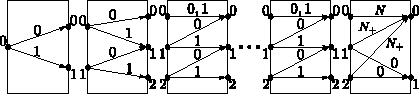
\includegraphics[scale=1.2]{SEA2026/Figures/OBDDs/CompleteOBDD.pdf}
    \caption{OBDD representing partial solutions to {\sc Vertex Cover} for the complete graph.}
    \label{fig:CompleteODD}
\end{figure}

\paragraph*{SDP-width of Complete Graphs}

We are now ready to establish the SDP-width of complete graphs.

\par\medskip
\noindent{\bf \cref{proposition:WidthClique}.}
{\it
Let $\dpcore$ be a DP-core solving {\sc Vertex Cover}, and let $\treedec$ be an
immediate tree decomposition of the complete graph $K_n$. Then
$\sw(\dpcore,\treedec)$ is bounded above by $\BigO(1)$.
}

\begin{proof}
Starting from a complete graph, we describe a sequence of OBDD constructions
corresponding to the introduction of a new vertex together with all edges
between this vertex and the existing clique.

The initial OBDD is shown in Figure~\ref{fig:CompleteODD}. Upon introducing a
vertex $u$, a new layer is added to initial OBDD $\ODD$ according to the operation
$\symbintrovertex{u}(\ODD)$. By definition, this operation introduces a layer without
increasing the width of the input OBDD producing $\ODD'$ . We then consider the introduction of an
edge $\{u,v\}$, where $v$ is a vertex of the clique. At this stage, the graph
consists of the clique together with a single vertex $u$ adjacent only to $v$. 

We first assume that the layer corresponding to $v$ appears before the layer
corresponding to $u$ in the variable order. We modify the OBDD $\ODD'$ at all
layers between positions $\activelabels[v]$ and $\activelabels[u]$ by introducing
a new state labeled~$3$, belonging to a new track. This track represents the
constraint that a string is simultaneously on \emph{thin ice} with respect to
the clique vertices and on \emph{thin ice} with respect to the newly introduced
vertex~$u$.

In particular, if a string in state~$3$ reads the value~$0$ at a layer
corresponding either to a clique vertex or to the layer corresponding to $v$,
then the string must be rejected and hence enter the reject track. Accordingly,
the transition $(2,0,1)$ at layer $\B_{\activelabels[v]}$, which previously
entered the thin ice track, is redirected to enter the new track~$3$; that is,
the transition $(2,0,3)$ replaces it.

At all subsequent layers with indices between $\activelabels[v]$ and
$\activelabels[u]$, transitions $(3,1,3)$ and $(3,0,0)$ are added. Finally, at
layer $\B_{\activelabels[u]}$, we add transitions $(3,0,0)$ and $(3,1,1)$. Reading
a~$0$ from state~$3$ at this layer causes the string to be rejected, since it
would violate the thin-ice constraint with respect to~$v$, while reading a~$1$
means that the string is now only on thin ice with respect to the clique
vertices.

The OBDD constructed above has width~$4$, and it is straightforward to verify
that it accepts exactly the encodings of partial solutions to {\sc Vertex Cover}
for a graph consisting of a clique together with a single additional vertex
connected to the clique by a single edge.

The case in which the new vertex~$u$ appears earlier in the variable order than
the clique vertex~$v$ is very similar. In this case, modifications are made to
the layers at positions between $\activelabels[u]$ and $\activelabels[v]$. Once
again, a new track~$3$ is introduced. This track represents a constraint on
vertex~$v$: if a string reaches state~$3$, then the value~$0$ was read at position
$\activelabels[u]$, and the string must be rejected if the layer corresponding to
$v$ is reached and the value~$0$ is read.

If the next layer does not correspond to~$v$ and the value~$0$ is read, then the
string enters the thin ice track, since the thin ice constraint subsumes the
requirement that the value~$1$ be read at layer $\activelabels[v]$ for the string
to encode a valid vertex cover. Accordingly, we modify layer
$\B_{\activelabels[u]}$ so that the transition $(2,0,2)$ is redirected to the new
track~$3$, that is, the transition $(2,0,3)$ replaces it. At subsequent layers,
we add transitions $(3,0,1)$, entering the thin ice track, and $(3,1,3)$,
remaining on track~$3$. Finally, at layer $\B_{\activelabels[v]}$, we add the
transitions $(3,0,0)$, entering the reject track when~$0$ is read, and $(3,1,2)$,
entering the accept track when~$1$ is read.

Generalizing to the introduction of an arbitrary number edge introductions is now starightforward. Upon subsequent edge introductions, At any layer corresponing to a vertex in the neighbourhood of $u$ appearing before $u$ in the variable ordering, we may further modify our OBDD by redirecting transition (2,0,1) to the new track 3. For neigbours of $u$ appearing after $u$ in the variable ordering, we redirect transistion (3,0,1) to to the reject rack (3,0,0). Thus for any consequetive edgesintrdutctions there exist an OBDD representig partial solutions to vertex cover for our given graph, taht is of width at most 4. We note that upon introducing all adges incident to vertex $u$ and th clique, we mayonce agian represent the patial solutions with an OBDD of size 3.

Generalizing this construction to the introduction of an arbitrary number of
edges is now straightforward. Upon subsequent edge introductions, for any layer
corresponding to a vertex in the neighborhood of $u$ that appears before $u$ in
the variable ordering, we further modify the OBDD by redirecting the transition
$(2,0,1)$ to the auxiliary track~$3$. For neighbors of $u$ that appear after $u$
in the variable ordering, we instead redirect the transition $(3,0,1)$ to the
reject track, that is, replace it by $(3,0,0)$. In this way, for any sequence of
consecutive edge introductions, there exists an OBDD representing the set of
partial solutions to {\sc Vertex Cover} for the current graph that has width at
most~$4$. We note that once all edges incident to vertex~$u$ and the clique have
been introduced, the set of partial solutions can again be represented by an
OBDD of width~$3$.

It remains to show that edges can be forgotten—and size components in the final
layer updated accordingly—without incurring a significant increase in the
minimum OBDD width. To see this, observe that forgetting a vertex~$u$ can be
handled by removing the layer corresponding to~$u$, deleting any redundant
transitions arising in the adjacent layers, and adding the transitions
$(2,1,1)$ and $(1,1,1)$ to the final layer. This yields an OBDD that correctly
represents the set of partial solutions produced by the operation
$\forgetvertex{u}$. When subsequently forgetting additional vertices, transitions
to the accepting state are incremented accordingly. Throughout this process, the
OBDD maintains width~$3$.

  

% The case for when new veretex $u$ appears earlier in the variable order thatn vlique vertex $v$ is very similar. I this case modification s are made to layers at positions between $\activelabels[u]$ and $\activelabels[v]$. Once again a new track is introduced, track 3. This track now represents the constraint ron vertices in th neighbouurhood of $u$, that is if a string reaches state 3 of the new track then itmeans that 0 was read at postion $\activelabels[v]$ and this string must go on to be rejected if the next layer corresponds to a neighbour of $u$ and 0 is read. Therefore we modify layer $\B_{\activelabels[u]}$ such that (2,0,2) is rediercted to new track 3 i.e. (2,0,3) replaces it. In subsequent layers, we ad transistion (3,0,0) (entering the reject track if 0 is read) and (3,1,3) (remaining on track 3) if the layer corresponds to a neighbour of $u$. we add transitions (3,0,1) enterig the thin ice tarck  and (3,1,3) remaining on track 3. At layer $\activelabels[v]$
\end{proof}

\paragraph*{SDP-width of Rook Graphs}

Bounding the SDP-width of rook graphs follows a strategy similar to that used
for complete graphs. We describe an OBDD representing the set of partial
solutions to {\sc Vertex Cover} for an arbitrary induced subgraph of the rook
graph $R_n$.

The OBDD consists of a reject state together with states indexed by pairs
$(rs,cs)$ of subsets of $[n]$. Intuitively, $rs$ records rows that are on thin
ice and $cs$ records columns that are on thin ice. The accept state corresponds
to $(\emptyset,\emptyset)$.

\medskip
\noindent\textbf{Transition structure.}

Let $(i,j)$ be the vertex corresponding to the first layer, that is,
$\activelabels[(i,j)] = 1$. The first layer contains a single left state
(the initial state). Reading~$1$ leads to the state $(\emptyset,\emptyset)$,
while reading~$0$ leads to the state $(\{i\},\{j\})$.

Now consider a later layer $\B_{\activelabels[(i,j)]}$ corresponding to a
vertex $(i,j)$, and let $(rs,cs)$ index the current state.

If $i \in rs$ or $j \in cs$, then reading~$0$ leads to rejection, while
reading~$1$ preserves the state:
\[
((rs,cs),1,(rs,cs))
\quad\text{and}\quad
((rs,cs),0,0).
\]

If $i \notin rs$ and $j \notin cs$, then reading~$0$ leads to
\[
(rs \cup \{i\},\, cs \cup \{j\}),
\]
while reading~$1$ preserves the state:
\[
((rs,cs),0,(rs \cup \{i\}, cs \cup \{j\}))
\quad\text{and}\quad
((rs,cs),1,(rs,cs)).
\]

\medskip
\noindent\textbf{The invariant $|rs| = |cs|$.}

Observe that the only transition that modifies the state is the transition
reading~$0$ in the case $i \notin rs$ and $j \notin cs$. In that case,
both row~$i$ and column~$j$ are added simultaneously.
Thus rows and columns are always introduced in pairs.

Since the initial state is $(\emptyset,\emptyset)$, it follows inductively that
along any accepting computation we always have
\[
|rs| = |cs|.
\]
Therefore, only pairs $(rs,cs)$ satisfying $|rs|=|cs|$ are reachable, and it
suffices to include only such states in the OBDD.

The number of such pairs equals
\[
\sum_{k=0}^{n} \binom{n}{k}^2
= \binom{2n}{n}
= \Theta\!\left(\frac{2^{2n}}{\sqrt{n}}\right).
\]
Hence the width of the constructed OBDD is
\[
\Theta\!\left(\frac{2^{2n}}{\sqrt{n}}\right).
\]



% \paragraph*{SDP-width of Rook Graphs}

% Bounding the SDP-width of rook graphs follows a strategy similar to that used
% for complete graphs. We begin by describing an OBDD representing the set of
% partial solutions to {\sc Vertex Cover} for an arbitrary induced subgraph of the
% rook graph $R_n$.

% We construct an OBDD of width $2^{\BigO(\sqrt{N})}$, where $N = n^2$, consisting
% of an accept track, a reject track, and a family of thin ice tracks indexed by
% pairs of sets $(rs,cs) \in 2^{[n]} \times 2^{[n]}$. Here, $rs$ represents a set of
% row indices and $cs$ represents a set of column indices. More precisely, if a
% string reaches the thin ice track indexed by $(rs,cs)$ (or simply the
% $(rs,cs)$-track), then reading the value~$0$ at the next layer causes the string
% to be rejected whenever the vertex associated with that layer lies in one of the
% rows in $rs$ or one of the columns in $cs$.

% Equivalently, if a string reaches the $(rs,cs)$-track, then for each $i \in rs$
% (respectively, each $j \in cs$), exactly one value~$0$ has already been read at a
% layer corresponding to a vertex in row~$i$ (respectively, column~$j$).

% We now define an OBDD representing the set of partial solutions to
% {\sc Vertex Cover} for an arbitrary induced subgraph of a rook graph.
% The transition structure of each layer is specified as follows.

% Let $(i,j)$ be the vertex corresponding to the first layer, that is,
% $\activelabels[(i,j)] = 1$. At this layer there is a single left state—the
% initial state—belonging to the accept track. The right states consist of one
% state for each pair of sets $(rs,cs) \in 2^{[n]} \times 2^{[n]}$, corresponding
% to the $(rs,cs)$-thin ice tracks, together with one state for the accept track.

% The layer $\B_{\activelabels[(i,j)]}$ contains one transition labeled~$1$
% from the initial state to the accept track, and one transition labeled~$0$
% from the initial state to the $(\{i\},\{j\})$-thin ice track.

% Now consider the transitions at layer $\B_{\activelabels[(i,j)]}$ for a vertex
% $(i,j)$ that is not assigned to the first layer. Let $(rs,cs)$ index a thin ice
% state.

% If $i \in rs$ or $j \in cs$, then reading the value~$0$ must lead to rejection,
% while reading the value~$1$ preserves the current constraint. Accordingly,
% layer $\B_{\activelabels[(i,j)]}$ contains transitions
% \[
% ((rs,cs),1,(rs,cs))
% \quad\text{and}\quad
% ((rs,cs),0,0)
% \]
% for each pair $(rs,cs)$ with $i \in rs$ or $j \in cs$.
% Intuitively, any string reaching the $(rs,cs)$-track is already on thin ice with
% respect to the rows in $rs$ and the columns in $cs$, and therefore reading~$0$
% at this layer would violate the vertex-cover constraint.

% On the other hand, if $i \notin rs$ and $j \notin cs$, then reading~$0$ leads to
% the thin ice track indexed by $(rs \cup \{i\},\, cs \cup \{j\})$, while reading~$1$
% leaves the state unchanged. That is, layer $\B_{\activelabels[(i,j)]}$ contains
% transitions
% \[
% ((rs,cs),0,(rs \cup \{i\}, cs \cup \{j\}))
% \quad\text{and}\quad
% ((rs,cs),1,(rs,cs)).
% \]
% Intuitively, reading~$0$ from such a state places future vertices on thin ice
% with respect to row~$i$ and column~$j$, whereas reading~$1$ imposes no additional
% constraints.



% \par\medskip
% \noindent{\bf \cref{proposition:SDPWidthRook}.}
% {\it 
% Let $\dpcore$ be a DP-core solving {\sc Vertex Cover} and let $\treedec$ be an immediate tree decomposition of the $N$-node rook graph $R_n$ (with $N = n^2$). Then $\sw(\dpcore, \treedec)$ is bounded above by $\Theta\!\left(\frac{2^{2n}}{\sqrt{n}}\right)$.
% }

% \begin{proof}
% We describe a sequence of OBDD constructions corresponding to the instructions
% of an immediate tree decomposition of $R_n$, and we show that throughout this
% sequence there exists an OBDD representing the current set of partial solutions
% whose width is bounded by
% $\Theta\!\left(\frac{2^{2n}}{\sqrt{n}}\right)$.

% \smallskip
% \noindent\textbf{State space and width bound.}
% We represent partial solutions using an OBDD whose non-reject states are indexed
% by pairs $(rs,cs)$ with $rs,cs \subseteq [n]$ and $|rs|=|cs|$, together with a
% single reject state. Intuitively, $(rs,cs)$ records the set of rows $rs$ and
% columns $cs$ that are currently \emph{on thin ice}: for each $i\in rs$
% (respectively $j\in cs$), exactly one vertex in row~$i$ (respectively
% column~$j$) has been assigned value~$0$ so far. The accept state is identified
% with $(\emptyset,\emptyset)$.

% The transition structure is defined so that the only way to change the index
% pair is by reading a $0$ at some vertex $(i,j)$ with $i\notin rs$ and $j\notin
% cs$, in which case both $i$ and $j$ are added simultaneously, moving to
% $(rs\cup\{i\}, cs\cup\{j\})$. Hence, starting from $(\emptyset,\emptyset)$, the
% invariant $|rs|=|cs|$ holds along all computations. Therefore, only states
% indexed by pairs $(rs,cs)$ with equal cardinality are reachable, and the number
% of such states is
% \[
% \sum_{k=0}^n \binom{n}{k}^2
% = \binom{2n}{n}
% = \Theta\!\left(\frac{2^{2n}}{\sqrt{n}}\right).
% \]
% Consequently, the width of our OBDD representation is bounded by
% $\Theta\!\left(\frac{2^{2n}}{\sqrt{n}}\right)$.

% \smallskip
% \noindent\textbf{Introduce-vertex steps.}
% Let $\ODD$ be an OBDD representing the current witness set at some node of
% $\treedec$. When a new vertex is introduced, the operation
% $\symbintrovertex{}$ inserts a new unconstraining layer and, by definition, does
% not increase the width of $\ODD$. Hence vertex introductions preserve the above
% width bound.

% \smallskip
% \noindent\textbf{Introduce-edge steps.}
% Consider the introduction of an edge between two already active vertices
% $x=(i,j)$ and $y=(i',j')$ in the rook graph, i.e., either $i=i'$ or $j=j'$.
% The operation $\symbintroedge{x}{y}$ is implemented as an intersection with a
% fixed filtering OBDD that removes exactly those assignments setting both
% endpoints to~$0$ (cf.\ the definition of $\symbintroedge{}{}$).
% Intersecting $\ODD$ with this filter yields an OBDD of width at most the product
% of widths, and subsequent minimization can only decrease width.

% In our setting, the filter enforces a constraint that is already captured by
% the thin-ice semantics: once a row (or column) is on thin ice, reading a second
% $0$ within that row (or column) leads to rejection. Introducing a rook edge
% between two vertices in a common row/column is therefore equivalent to
% forbidding the simultaneous assignment of $0$ to both endpoints, which is
% realized by redirecting a bounded number of transitions into the reject state
% (or, equivalently, by refining the thin-ice state space by at most a constant
% factor per introduced vertex). Thus, during any sequence of edge introductions
% incident to a newly introduced vertex, we can maintain an equivalent OBDD whose
% states are still indexed by pairs $(rs,cs)$ with $|rs|=|cs|$, and whose width
% remains bounded by
% $\Theta\!\left(\frac{2^{2n}}{\sqrt{n}}\right)$.
% (Full transition-level details are given in Appendix~\ref{...}.)

% \smallskip
% \noindent\textbf{Forget-vertex steps.}
% Finally, consider forgetting a vertex $x=(i,j)$. The DP-core operation
% $\forgetvertex{x}$ removes the corresponding bit from the witness string and
% increments the size component by the value assigned to $x$. Symbolically, this
% is implemented by contracting away the layer for $x$ and updating the size
% labels in the final layer accordingly (cf.\ Appendix~\ref{subsec:FrgProof}).
% This operation does not increase the number of $(rs,cs)$-indexed states and
% therefore preserves the width bound.

% \smallskip
% Combining the above, at every node of the immediate decomposition $\treedec$
% there exists an OBDD representing the set of partial solutions whose width is
% bounded by $\Theta\!\left(\frac{2^{2n}}{\sqrt{n}}\right)$. Hence
% $\sw(\dpcore,\treedec)$ is bounded above by
% $\Theta\!\left(\frac{2^{2n}}{\sqrt{n}}\right)$, as claimed.
% \end{proof}


\par\medskip
\noindent{\bf \cref{proposition:SDPWidthRook}.}
{\it
Let $\dpcore$ be a DP-core solving {\sc Vertex Cover} and let $\treedec$ be an
immediate tree decomposition of the $N$-vertex rook graph $R_n$ (with $N=n^2$).
Then $\sw(\dpcore,\treedec)$ is bounded above by
$\Theta\!\left(\frac{2^{2n}}{\sqrt{n}}\right)$.
}

\begin{proof}
Fix a node $p$ of $\treedec$ with active-label map $\activelabels$ and let
$G_p$ denote the graph induced by the currently active vertices in the rook
graph (equivalently, since $\treedec$ is immediate and edges are introduced as
soon as both endpoints are active, $G_p$ contains exactly the rook edges whose
endpoints are active at $p$).

We show that for every such node $p$ there exists an OBDD $\ODD_p$ recognizing
exactly the witness set produced by the {\sc Vertex Cover} DP-core at $p$, and
whose states are indexed by the same family of pairs $(rs,cs)$ as in the
transition structure defined above (together with the reject state). Since the
number of reachable such pairs has been bounded immediately preceding the
proposition, it follows that $\ODD_p$ has width
$\Theta\!\left(\frac{2^{2n}}{\sqrt{n}}\right)$, and hence
$\sw(\dpcore,\treedec)$ is bounded above by this value.

\smallskip
\noindent\textbf{Canonical rook-OBDD for an active set.}
For any active-label map $\activelabels$, define the \emph{canonical rook-OBDD}
$\ODD(\activelabels)$ to be the OBDD whose layers are indexed by
$1,\dots,|\activelabels|$ and whose state set consists of:
(i) one reject state (denoted $0$), and (ii) one state for each pair
$(rs,cs)$ with $rs,cs \subseteq [n]$ and $|rs|=|cs|$.
The initial state is $(\emptyset,\emptyset)$, and the transition relation at
layer $\B_{\activelabels[(i,j)]}$ is exactly as specified in the ``Transition
structure'' paragraph above. (Equivalently, $(\emptyset,\emptyset)$ plays the
role of the accept-track state.)

The final layer $\B_{|\activelabels|+1}$ is defined as in the {\sc Vertex Cover}
SDP-core: for each left state $q$ and each size $t \in \dbset{|V|}$ it contains a
transition labeled $t$ from $q$ to the accept state iff $t$ equals the number of
vertices assigned value $1$ among the forgotten vertices so far (as maintained
by the DP-core), and otherwise it goes to the reject state. (This is the same
size-accounting convention used throughout the appendix; we omit repetition.)

\smallskip
\noindent\textbf{Correctness invariant.}
We prove by induction over the nodes of $\treedec$ that for each node $p$ the
witness set $\Witnesses(p)$ computed by the {\sc Vertex Cover} DP-core equals
$\Lang(\ODD_p)$ for some OBDD $\ODD_p$ obtainable from $\ODD(\activelabels)$ by
size-label adjustments only (i.e., without changing the \emph{string} acceptance
behavior determined by the $(rs,cs)$-indexed transition structure).

\smallskip
\noindent\textbf{Leaf nodes.}
At a leaf, $\Witnesses(p)=\leaf$ and the OBDD is exactly the OBDD defined by
$\symbleaf$. This matches the canonical construction with no active vertices.

\smallskip
\noindent\textbf{Introduce-vertex nodes.}
Let $p$ be an introduce-vertex node introducing a vertex $x=(i,j)$ and let $p'$
be its child. By induction, $\Witnesses(p')=\Lang(\ODD_{p'})$ for some $\ODD_{p'}$
of the required form. The symbolic operation $\symbintrovertex{x}$ inserts a
fresh layer at position $\activelabels[x]$ that reads $0$ and $1$ and otherwise
acts as the identity on states. This does not change the state set and hence
preserves the width bound. Let the resulting OBDD be $\ODD'$.

\smallskip
\noindent\textbf{Introduce-edge nodes.}
Let $p$ be an introduce-edge node introducing an edge $\{x,y\}$, where
$x=(i,j)$ and $y=(i',j')$ are active and adjacent in $R_n$ (so either $i=i'$ or
$j=j'$), and let $p'$ be its child. By induction, $\Witnesses(p')$ is recognized
by an OBDD $\ODD_{p'}$ whose string acceptance is governed by the canonical
$(rs,cs)$ transition structure on the current active set.

By definition of {\sc Vertex Cover}, introducing the edge $\{x,y\}$ removes
exactly those witnesses that assign $0$ to both $x$ and $y$. We show that the
canonical transition structure enforces precisely this constraint at the moment
the edge becomes present in $G_p$.

Assume w.l.o.g.\ that $\activelabels[x] < \activelabels[y]$ in the variable
order. Consider any run of $\ODD_{p'}$ up to (and including) layer
$\B_{\activelabels[x]}$. If the input assigns $0$ to $x=(i,j)$, then by the
canonical rule the run moves from some state $(rs,cs)$ with $i\notin rs$ and
$j\notin cs$ to the state $(rs\cup\{i\}, cs\cup\{j\})$. In particular, after
reading $x=0$ we have $i \in rs$ and $j \in cs$ in the current state component.

Now consider the later layer $\B_{\activelabels[y]}$:
\begin{itemize}
\item If $y$ shares row with $x$ (i.e., $i=i'$), then $i \in rs$ holds at this
layer whenever $x=0$ was read earlier. Hence, by the canonical rule, reading
$y=0$ forces a transition to the reject state. Thus assignments with $x=0$ and
$y=0$ are rejected.
\item If $y$ shares column with $x$ (i.e., $j=j'$), then analogously $j \in cs$
holds whenever $x=0$ was read earlier, and reading $y=0$ forces rejection.
\end{itemize}

Conversely, if the input does \emph{not} assign $0$ to both endpoints, then at
most one of the conditions ``$i\in rs$'' or ``$j\in cs$'' relevant for the edge
can be triggered by the earlier endpoint, and the canonical rule permits the
later endpoint to be read consistently (in particular, if the later endpoint is
read as $1$, the state does not change; if it is read as $0$, it is permitted
exactly when neither the corresponding row nor column is already in thin ice).

Therefore, intersecting with the edge-filter OBDD
$\ODD^{\{x,y\}}$ removes exactly those strings with $x=y=0$, and the minimized
result recognizes exactly the witness set after introducing $\{x,y\}$. Moreover,
the minimized result is recognized by an OBDD of the canonical $(rs,cs)$ form for
the updated active induced graph $G_p$, since the canonical transition structure
enforces all rook edges among active vertices in the same row or column. Denote
this minimized OBDD by $\ODD_p$.

\smallskip
\noindent\textbf{Forget-vertex nodes.}
Let $p$ be a forget-vertex node forgetting a vertex $x=(i,j)$ and let $p'$ be
its child. By induction, $\Witnesses(p')=\Lang(\ODD_{p'})$ for an OBDD of the
canonical $(rs,cs)$ form with the appropriate size-accounting in the final layer.

The symbolic operation $\symbforgetvertex{x}$ is implemented by (i) separating
the language of $\ODD_{p'}$ into the sublanguages with $x=0$ and with $x=1$,
(ii) incrementing the size labels by $1$ on the $x=1$ branch, (iii) taking the
union, and (iv) contracting away the layer $\B_{\activelabels[x]}$ (as specified
in Appendix~\ref{subsec:FrgProof}). None of these steps introduces new
$(rs,cs)$-indexed states. Hence the resulting minimized OBDD again has the
canonical state space and satisfies the same width bound.

Here immediacy is used as follows: a vertex is forgotten only after all its
incident edges have been introduced, so no future constraint depends on the
value of $x$. Thus contracting away the layer for $x$ yields exactly the
DP-core witness update and does not require introducing additional state.

\smallskip
\noindent\textbf{Join nodes.}
Let $p$ be a join node with children $p_1,p_2$ sharing the same active label map
$\activelabels$. By induction, $\Witnesses(p_1)$ and $\Witnesses(p_2)$ are
recognized by OBDDs $\ODD_{p_1}$ and $\ODD_{p_2}$ over the canonical $(rs,cs)$
transition structure (with possibly different size labels in the final layer).
The symbolic join operation is performed as defined in the appendix ``Join''
paragraph: it aggregates size components for witnesses with identical string
components using the intermediate OBDDs $\ODD^{\scriptcap}$ and $\ODD^{\scriptcup}$
and returns $\minODD(\ODD^{\scriptcap}\cup\ODD^{\scriptcup})$. This construction
does not alter the underlying string-acceptance transition structure, only the
size labels in the final layer. Hence it preserves the canonical state space and
the width bound.

\smallskip
We have shown that at every node $p$ of $\treedec$ the witness set computed by
the {\sc Vertex Cover} DP-core is recognized by an OBDD whose state space is the
canonical $(rs,cs)$ family (plus reject), and therefore has width bounded above
by $\Theta\!\left(\frac{2^{2n}}{\sqrt{n}}\right)$. This establishes the claimed
upper bound on $\sw(\dpcore,\treedec)$.
\end{proof}
